\documentclass[tikz,border=4pt]{standalone}
\usepackage[scheme=plain]{ctex}
\usepackage{anyfontsize,pgfplots,siunitx}
\usetikzlibrary{arrows.meta,calc,decorations.markings,decorations.pathmorphing,positioning}
% 各卷共用的数学记号。课程专用记号见相应的主入口。
\RequirePackage{amsmath,amssymb,bm,upgreek}

% 数集与函数空间
\newcommand*{\NN}{\mathbb{N}}
\newcommand*{\ZZ}{\mathbb{Z}}
\newcommand*{\QQ}{\mathbb{Q}}
\newcommand*{\RR}{\mathbb{R}}
\newcommand*{\CC}{\mathbb{C}}
\newcommand*{\FF}{\mathbb{F}}
\newcommand*{\cont}{\mathcal{C}}  % 连续函数空间，\cont^k 表示 k 次连续可微
\newcommand*{\poly}{\mathcal{P}}  % \poly_n 中多项式的次数至多为 n

% 微分与常数。文本中的无点 i 和字母下加点另有明确的命令。
\NewCommandCopy{\dotlessi}{\i}
\NewCommandCopy{\dotbelow}{\d}
\renewcommand*{\i}{\mathrm{i}}
\newcommand*{\nd}{\mathrm{d}}
\renewcommand*{\d}{\mathop{}\!\mathrm{d}}
\newcommand*{\e}{\mathop{}\!\mathrm{e}}
\newcommand*{\const}{\mathrm{const}}
\newcommand*{\vd}{\mathop{}\!\delta}  % 变分、依赖过程的热量或功的微元
\newcommand*{\p}{\partial}
\newcommand{\dd}[2][]{\frac{\d^{#1}}{\nd{#2}^{#1}}}
\newcommand{\dv}[3][]{\frac{\d^{#1}#2}{\nd{#3}^{#1}}}
\newcommand{\pp}[2][]{\frac{\p^{#1}}{\p{#2}^{#1}}}
\newcommand{\pv}[3][]{\frac{\p^{#1}#2}{\p{#3}^{#1}}}
\newcommand{\pw}[3]{\frac{\p^2{#1}}{\p{#2}\p{#3}}}

% 函数与算符
\let\Re\relax
\let\Im\relax
\DeclareMathOperator{\Re}{Re}
\DeclareMathOperator{\Im}{Im}
\DeclareMathOperator{\sech}{sech}
\DeclareMathOperator{\csch}{csch}
\DeclareMathOperator{\sinc}{sinc}
\DeclareMathOperator{\sgn}{sgn}
\DeclareMathOperator{\id}{id}
\DeclareMathOperator{\PV}{PV}
\DeclareMathOperator{\FT}{\mathcal{F}}
\DeclareMathOperator{\Beta}{B}
\DeclareMathOperator*{\argmin}{arg\,min}
\DeclareMathOperator*{\argmax}{arg\,max}
\newcommand*{\bigo}{\mathcal{O}}
\newcommand*{\intR}{\int_{-\infty}^\infty}
\newcommand*{\intRplus}{\int_0^\infty}

% 矢量、线性代数与场算符
\newcommand*{\hatbm}[1]{\hat{\bm{#1}}} % 带帽的粗体符号，含义随卷定义
\newcommand*{\dotbm}[1]{\dot{\bm{#1}}}
\newcommand*{\uvec}[1]{\mathop{}\!\hatbm{#1}}  % 系数后自动留薄空；单独取负写 -{\uvec n}
\newcommand*{\grad}{\nabla}
\renewcommand*{\div}{\nabla\cdot}
\newcommand*{\curl}{\nabla\times}
\newcommand*{\laplacian}{\nabla^2}
\DeclareMathOperator{\rank}{rank}
\DeclareMathOperator{\diag}{diag}
\DeclareMathOperator{\tr}{tr}
\DeclareMathOperator{\Span}{span}
\DeclareMathOperator{\nullsp}{N}
\DeclareMathOperator{\colsp}{C}
\newcommand*{\transp}{^\top}
\newcommand*{\conj}{^\ast}
\newcommand*{\adjoint}{^\dagger}
\newcommand*{\inv}{^{-1}}

% 概率、统计与物理量
\renewcommand*{\P}{\operatorname{P}}  % 段落符号 ¶ 可用 \textparagraph
\DeclareMathOperator{\E}{E}
\DeclareMathOperator{\Var}{Var}
\DeclareMathOperator{\BinDist}{Bin}
\DeclareMathOperator{\NormalDist}{N}
\newcommand*{\avg}[1]{\overline{#1}}
\newcommand*{\NA}{N_{\mathrm{A}}}
\newcommand*{\kB}{k_{\mathrm{B}}}
\newcommand*{\muB}{\mu_{\mathrm{B}}}
\newcommand*{\Ek}{E_{\mathrm{k}}}
\newcommand*{\FWHM}{\mathrm{FWHM}}
\newcommand*{\electron}{\mathrm{e}}       % 粒子标签，如 m_\electron
\newcommand*{\proton}{\mathrm{p}}
\newcommand*{\nucleus}{\mathrm{N}}
\newcommand*{\excitedstate}{\mathrm{e}}
\newcommand*{\groundstate}{\mathrm{g}}
\newcommand*{\CM}{\mathrm{CM}}
\newcommand*{\transv}{\mathrm t}  % 横向分量或模式的标签
\newcommand*{\longit}{\mathrm l}  % 纵向分量或模式的标签
\newcommand*{\electric}{\mathrm e}
\newcommand*{\magnetic}{\mathrm m}
\newcommand*{\incident}{\mathrm i}
\newcommand*{\initial}{\mathrm i}
\newcommand*{\final}{\mathrm f}
\newcommand*{\hi}{\mathrm{hi}}
\newcommand*{\lo}{\mathrm{lo}}
\newcommand*{\eff}{\mathrm{eff}}
\newcommand*{\tot}{\mathrm{tot}}

% 括号与 Dirac 记号。显式声明让公式预览也能读到每个尺寸的命令。
\newcommand{\abs}[1]{\lvert#1\rvert}
\newcommand{\bigabs}[1]{\bigl\lvert#1\bigr\rvert}
\newcommand{\Bigabs}[1]{\Bigl\lvert#1\Bigr\rvert}
\newcommand{\biggabs}[1]{\biggl\lvert#1\biggr\rvert}
\newcommand{\Biggabs}[1]{\Biggl\lvert#1\Biggr\rvert}

\newcommand{\norm}[1]{\lVert#1\rVert}
\newcommand{\bignorm}[1]{\bigl\lVert#1\bigr\rVert}
\newcommand{\Bignorm}[1]{\Bigl\lVert#1\Bigr\rVert}
\newcommand{\biggnorm}[1]{\biggl\lVert#1\biggr\rVert}
\newcommand{\Biggnorm}[1]{\Biggl\lVert#1\Biggr\rVert}

\newcommand{\eval}[1]{{#1}\rvert}
\newcommand{\bigeval}[1]{{#1}\bigr\rvert}
\newcommand{\Bigeval}[1]{{#1}\Bigr\rvert}
\newcommand{\biggeval}[1]{{#1}\biggr\rvert}
\newcommand{\Biggeval}[1]{{#1}\Biggr\rvert}

\newcommand{\floor}[1]{\lfloor#1\rfloor}
\newcommand{\bigfloor}[1]{\bigl\lfloor#1\bigr\rfloor}
\newcommand{\Bigfloor}[1]{\Bigl\lfloor#1\Bigr\rfloor}
\newcommand{\biggfloor}[1]{\biggl\lfloor#1\biggr\rfloor}
\newcommand{\Biggfloor}[1]{\Biggl\lfloor#1\Biggr\rfloor}

\newcommand{\ceil}[1]{\lceil#1\rceil}
\newcommand{\bigceil}[1]{\bigl\lceil#1\bigr\rceil}
\newcommand{\Bigceil}[1]{\Bigl\lceil#1\Bigr\rceil}
\newcommand{\biggceil}[1]{\biggl\lceil#1\biggr\rceil}
\newcommand{\Biggceil}[1]{\Biggl\lceil#1\Biggr\rceil}

\newcommand{\ave}[1]{\langle#1\rangle}
\newcommand{\bigave}[1]{\bigl\langle#1\bigr\rangle}
\newcommand{\Bigave}[1]{\Bigl\langle#1\Bigr\rangle}
\newcommand{\biggave}[1]{\biggl\langle#1\biggr\rangle}
\newcommand{\Biggave}[1]{\Biggl\langle#1\Biggr\rangle}

\newcommand{\set}[2]{\{#1\,\vert\,#2\}}
\newcommand{\bigset}[2]{\bigl\{#1\,\big\vert\,#2\bigr\}}
\newcommand{\Bigset}[2]{\Bigl\{#1\,\Big\vert\,#2\Bigr\}}
\newcommand{\biggset}[2]{\biggl\{#1\,\bigg\vert\,#2\biggr\}}
\newcommand{\Biggset}[2]{\Biggl\{#1\,\Bigg\vert\,#2\Biggr\}}

\newcommand{\division}[2]{{#1}/{#2}}
\newcommand{\bigdivision}[2]{{#1}\big/{#2}}
\newcommand{\Bigdivision}[2]{{#1}\Big/{#2}}
\newcommand{\biggdivision}[2]{{#1}\bigg/{#2}}
\newcommand{\Biggdivision}[2]{{#1}\Bigg/{#2}}

\newcommand{\inp}[2]{\langle#1,#2\rangle}
\newcommand{\biginp}[2]{\bigl\langle#1,#2\bigr\rangle}
\newcommand{\Biginp}[2]{\Bigl\langle#1,#2\Bigr\rangle}
\newcommand{\bigginp}[2]{\biggl\langle#1,#2\biggr\rangle}
\newcommand{\Bigginp}[2]{\Biggl\langle#1,#2\Biggr\rangle}

\newcommand{\bra}[1]{\langle#1\rvert}
\newcommand{\bigbra}[1]{\bigl\langle#1\bigr\rvert}
\newcommand{\Bigbra}[1]{\Bigl\langle#1\Bigr\rvert}
\newcommand{\biggbra}[1]{\biggl\langle#1\biggr\rvert}
\newcommand{\Biggbra}[1]{\Biggl\langle#1\Biggr\rvert}

\newcommand{\ket}[1]{\lvert#1\rangle}
\newcommand{\bigket}[1]{\bigl\lvert#1\bigr\rangle}
\newcommand{\Bigket}[1]{\Bigl\lvert#1\Bigr\rangle}
\newcommand{\biggket}[1]{\biggl\lvert#1\biggr\rangle}
\newcommand{\Biggket}[1]{\Biggl\lvert#1\Biggr\rangle}

\newcommand{\braket}[2]{\langle#1\vert#2\rangle}
\newcommand{\bigbraket}[2]{\bigl\langle#1\big\vert#2\bigr\rangle}
\newcommand{\Bigbraket}[2]{\Bigl\langle#1\Big\vert#2\Bigr\rangle}
\newcommand{\biggbraket}[2]{\biggl\langle#1\bigg\vert#2\biggr\rangle}
\newcommand{\Biggbraket}[2]{\Biggl\langle#1\Bigg\vert#2\Biggr\rangle}

\newcommand{\mel}[3]{\langle#1\vert#2\vert#3\rangle}
\newcommand{\bigmel}[3]{\bigl\langle#1\big\vert#2\big\vert#3\bigr\rangle}
\newcommand{\Bigmel}[3]{\Bigl\langle#1\Big\vert#2\Big\vert#3\Bigr\rangle}
\newcommand{\biggmel}[3]{\biggl\langle#1\bigg\vert#2\bigg\vert#3\biggr\rangle}
\newcommand{\Biggmel}[3]{\Biggl\langle#1\Bigg\vert#2\Bigg\vert#3\Biggr\rangle}

\newcommand{\ketbra}[2]{\lvert#1\rangle\langle#2\rvert}
\newcommand{\bigketbra}[2]{\bigl\lvert#1\bigr\rangle\bigl\langle#2\bigr\rvert}
\newcommand{\Bigketbra}[2]{\Bigl\lvert#1\Bigr\rangle\Bigl\langle#2\Bigr\rvert}
\newcommand{\biggketbra}[2]{\biggl\lvert#1\biggr\rangle\biggl\langle#2\biggr\rvert}
\newcommand{\Biggketbra}[2]{\Biggl\lvert#1\Biggr\rangle\Biggl\langle#2\Biggr\rvert}

% 兼容旧版笔记中的内积与外积命令。
\let\brkt\braket
\let\bigbrkt\bigbraket
\let\Bigbrkt\Bigbraket
\let\biggbrkt\biggbraket
\let\Biggbrkt\Biggbraket
\let\ktbr\ketbra
\let\bigktbr\bigketbra
\let\Bigktbr\Bigketbra
\let\biggktbr\biggketbra
\let\Biggktbr\Biggketbra

\newcommand{\bigp}[1]{\bigl(#1\bigr)}
\newcommand{\Bigp}[1]{\Bigl(#1\Bigr)}
\newcommand{\biggp}[1]{\biggl(#1\biggr)}
\newcommand{\Biggp}[1]{\Biggl(#1\Biggr)}

\newcommand{\bigb}[1]{\bigl[#1\bigr]}
\newcommand{\Bigb}[1]{\Bigl[#1\Bigr]}
\newcommand{\biggb}[1]{\biggl[#1\biggr]}
\newcommand{\Biggb}[1]{\Biggl[#1\Biggr]}

\newcommand{\bigB}[1]{\bigl\{#1\bigr\}}
\newcommand{\BigB}[1]{\Bigl\{#1\Bigr\}}
\newcommand{\biggB}[1]{\biggl\{#1\biggr\}}
\newcommand{\BiggB}[1]{\Biggl\{#1\Biggr\}}

% 公式排版
% 方程组的内容是一个 aligned 块，左花括号随整组方程的高度伸展。
\newcommand{\eqnset}[1]{\left\{#1\right.}
\newcommand{\fracdisp}[2]{\frac{\displaystyle #1}{\displaystyle #2}}
\newcommand*{\vs}{\mathord{\text{–}}}
\newcommand*{\otherwise}{\text{otherwise}}
\newcommand*{\qqquad}{\qquad\quad}
\newcommand*{\qqqquad}{\qquad\qquad}

\renewcommand*{\le}{\leqslant}
\renewcommand*{\leq}{\leqslant}
\renewcommand*{\ge}{\geqslant}
\renewcommand*{\geq}{\geqslant}

% 中文正文与图册用帽号区分量子算符。
\newcommand*{\op}[1]{\hat{#1}}

% 单电子轨道与分波
\newcommand*{\orbitalS}{\mathrm{s}}
\newcommand*{\orbitalP}{\mathrm{p}}
\newcommand*{\orbitalD}{\mathrm{d}}
\newcommand*{\orbitalF}{\mathrm{f}}

% 原子光谱项
\newcommand*{\termS}{\mathrm{S}}
\newcommand*{\termP}{\mathrm{P}}
\newcommand*{\termD}{\mathrm{D}}
\newcommand*{\termF}{\mathrm{F}}
\newcommand*{\EHartree}{E_{\mathrm h}}

% 自旋单态
\newcommand*{\singlet}{\mathrm{s}}

% 复合系统、仪器与读数
\newcommand*{\syslabel}{\mathrm{S}}
\newcommand*{\detlabel}{\mathrm{D}}
\newcommand*{\envlabel}{\mathrm{E}}
\newcommand*{\sysenv}{\mathrm{SE}}
\newcommand*{\ancilla}{\mathrm{A}}
\newcommand*{\subsysA}{\mathrm{A}}
\newcommand*{\subsysB}{\mathrm{B}}
\newcommand*{\subsysAB}{\mathrm{AB}}
\newcommand*{\leftLabel}{\mathrm{L}}
\newcommand*{\rightLabel}{\mathrm{R}}
\newcommand*{\detection}{\mathrm{det}}
\newcommand*{\bg}{\mathrm{bg}}

% 时间演化与相互作用
\newcommand*{\picS}{\mathrm{S}}
\newcommand*{\picH}{\mathrm{H}}
\newcommand*{\picI}{\mathrm{I}}
\newcommand*{\rotframe}{\mathrm{R}}
\newcommand*{\rabiLabel}{\mathrm{R}}
\newcommand*{\dyn}{\mathrm{dyn}}
\newcommand*{\eqm}{\mathrm{eq}}
\newcommand*{\spreadLabel}{\mathrm{s}}
\newcommand*{\reflected}{\mathrm{r}}
\newcommand*{\barrierLabel}{\mathrm{b}}
\newcommand*{\boundLabel}{\mathrm{b}}

% 光谱与带电粒子动力学
\newcommand*{\spin}{\mathrm{s}}
\newcommand*{\zeemanLabel}{\mathrm{Z}}
\newcommand*{\diracLabel}{\mathrm{D}}
\newcommand*{\atomH}{\mathrm{H}}
\newcommand*{\keplerLabel}{\mathrm{K}}
\newcommand*{\retarding}{\mathrm{r}}
\newcommand*{\cyclotron}{\mathrm{c}}
\newcommand*{\orbitctr}{\mathrm{c}}

\colorlet{ink}{blue!20!black}
\colorlet{curve}{teal!74!black}
\colorlet{amplitude}{teal!75!black}
\colorlet{shortwave}{blue!70!black}
\colorlet{longwave}{orange!85!black}
\colorlet{balmerAlpha}{red!74!black}
\colorlet{balmerBeta}{teal!85!black}
\definecolor{matrixpale}{HTML}{DBE7F2}
\definecolor{matrixblue}{HTML}{6D90B7}
\definecolor{matrixnavy}{HTML}{1F4272}
\definecolor{matrixcoral}{HTML}{E6A396}
\definecolor{matrixbrick}{HTML}{A63F44}
% 图按正文中的印刷尺寸绘制。坐标可单独缩放，文字统一用小五号。
\tikzset{
    every picture/.append style={font=\zihao{-5}},
    matrix cell/.style={draw=black!18,line width=.2pt},
    radiation/.style={thick,->,decorate,
        decoration={snake,amplitude=.65mm,segment length=#1,post length=1.4mm}},
    radiation/.default=3mm
}

% Blackbody models and spectra (Izaak Neutelings, March 2019).
\tikzstyle{cavity radiation}=[-{Latex[length=2,width=1.5]},red!95!black!50,opacity=0.7,very thin,decorate,
                       decoration={snake,amplitude=0.7,segment length=2,post length=2}]

\pgfplotsset{
  compat=1.13, % TikZ coordinates <-> axes coordinates
  colormap={matrix sequential}{
    color(0cm)=(matrixpale); color(1cm)=(matrixblue); color(2cm)=(matrixnavy)
  },
  colormap={matrix signed}{
    color(0cm)=(matrixbrick); color(1cm)=(matrixcoral); color(2cm)=(white);
    color(3cm)=(matrixblue); color(4cm)=(matrixnavy)
  },
  /pgf/number format/1000 sep={},
  legend image code/.code={
    \draw[mark repeat=2,mark phase=2]
    plot coordinates {(0cm,0cm) (0.22cm,0cm) (0.44cm,0cm)};%
  }
}

% TikZ 的矩形色条显示色阶定义的中央一半，与上面的矩阵配色一致。
\pgfdeclareverticalshading{matrix signed}{100bp}{
    color(0bp)=(matrixbrick); color(25bp)=(matrixbrick);
    color(37.5bp)=(matrixcoral); color(50bp)=(white); color(62.5bp)=(matrixblue);
    color(75bp)=(matrixnavy); color(100bp)=(matrixnavy)
}

% redraw axis on top
\makeatletter \newcommand{\pgfplotsdrawaxis}{\pgfplots@draw@axis} \makeatother
\pgfplotsset{axis line on top/.style={after end axis/.append code={\pgfplotsdrawaxis}}
}

% CUSTOM COLORS
% See https://tikz.net/blackbody_color/
\definecolor{1000K}{rgb}{1,0.0337,0}
\definecolor{2000K}{rgb}{1,0.2647,0.0033}
\definecolor{3000K}{rgb}{1,0.4870,0.1411}
\definecolor{4000K}{rgb}{1,0.6636,0.3583}
\definecolor{5000K}{rgb}{1,0.7992,0.6045}
\definecolor{6000K}{rgb}{1,0.9019,0.8473}
\definecolor{8000K}{rgb}{0.7874,0.8187,1}
\definecolor{10000K}{rgb}{0.6268,0.7039,1}
\pgfdeclareverticalshading{rainbow}{100bp}{
  color(0bp)=(red); color(25bp)=(red); color(35bp)=(yellow);
  color(45bp)=(green); color(55bp)=(cyan); color(65bp)=(blue);
  color(75bp)=(violet); color(100bp)=(violet)
}
\colorlet{myred}{red!70!black}
\colorlet{mygreen}{green!70!black}
\colorlet{mydarkgreen}{green!55!black}

% PLANCK & RAYLEIGH-JEANS
% 2hc^2/lambda^5 = 2 * 6.62607015e-34 * 299792458^2
%                = 1.191042972e-16
% For wavelength in nm and spectral radiance in uW sr^-1 m^-2 nm^-1: 1.191042972e26
%  hc/k lambda T = 6.62607015e-34*299792458/(1.38064852e-23)
%                = 0.01438777378
%         m -> nm: 0.01438777378e9
% 2ckT/lambda^4  = 2 * 299792458 * 1.38064852e-23
%                = 8.278160269e-15
% In the same units: 8.278160269e18
\pgfmathdeclarefunction{planck}{2}{%
  \pgfmathparse{1.191042972e26/(#1^5)/(exp(0.01439e9/(#1*#2))-1)}%
}
\pgfmathdeclarefunction{rayleighjeans}{2}{%
  \pgfmathparse{8.278160269e18*#2/(#1^4)}%
}
\pgfmathdeclarefunction{wien}{2}{%
  \pgfmathparse{1.191042972e26/(#1^5)*exp(-0.01439e9/(#1*#2))}%
}
\pgfmathdeclarefunction{lampeak}{1}{% % Wien's displacement law
  \pgfmathparse{2.898e6/#1}%
}

\pgfdeclareverticalshading{blackbody}{100}{
  rgb(0)=(0,0,0);
  rgb(25)=(0,0,0);
  rgb(25+50/11*1)=(1,0.0337,0);
  rgb(25+50/11*2)=(1,0.2647,0.0033);
  rgb(25+50/11*3)=(1,0.4870,0.1411);
  rgb(25+50/11*4)=(1,0.6636,0.3583);
  rgb(25+50/11*5)=(1,0.7992,0.6045);
  rgb(25+50/11*6)=(1,0.9019,0.8473);
  rgb(25+50/11*6.5)=(1,1,1);
  rgb(25+50/11*7)=(0.9337,0.9150,1);
  rgb(25+50/11*8)=(0.7874,0.8187,1);
  rgb(25+50/11*9)=(0.6925,0.7522,1);
  rgb(25+50/11*10)=(0.6268,0.7039,1);
  rgb(75)=(0.3277,0.5022,1);
  rgb(100)=(0.3277,0.5022,1)
}

\begin{document}

% 绪论
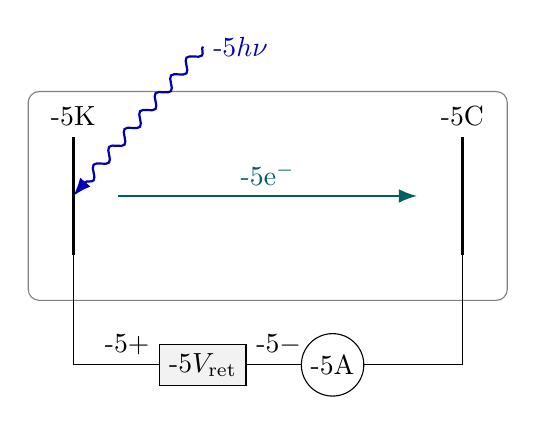
\begin{tikzpicture}[scale=1.3,>=Latex,beam/.style={teal!75!black,thick,->}]
    \label{photoelectric-cell}
    \def\gap{3.8} \def\plate{.58} \def\wall{.44} \def\wireY{-1.65}
    \coordinate (K) at (0,0);
    \coordinate (C) at (\gap,0);
    \draw[rounded corners,black!50] (-\wall,-\plate-\wall) rectangle (\gap+\wall,\plate+\wall);
    \foreach \electrode in {K,C}{
        \draw[very thick] ($(\electrode)+(0,-\plate)$) -- ($(\electrode)+(0,\plate)$)
            node[above] {$\mathrm{\electrode}$};
    }
    \draw[radiation,shortwave] (\gap/3,\plate+2*\wall) node[right] {$h\nu$} -- (K);
    \draw[beam] (\wall,0) -- node[above] {$\electron^-$} (\gap-\wall,0);
    \node[draw,fill=black!5] (bias) at (\gap/3,\wireY) {$V_{\rm ret}$};
    \node[draw,circle,inner sep=2pt] (meter) at (2*\gap/3,\wireY) {A};
    \draw (0,-\plate) |- (bias.west) node[above left] {$+$};
    \draw (bias.east) node[above right] {$-$} -- (meter.west);
    \draw (meter.east) -| (\gap,-\plate);
\end{tikzpicture}

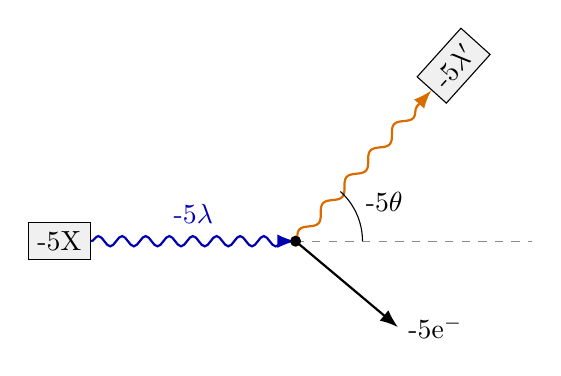
\begin{tikzpicture}[>=Latex]
    \label{compton-geometry}
    \def\arm{3} \def\thetaOut{48} \def\recoilAngle{40} \def\arcRadius{.85}
    \node[draw,fill=black!6] (source) at (-\arm,0) {X};
    \node[draw,fill=black!6,rotate=\thetaOut] (spectrometer) at (\thetaOut:\arm) {$\lambda'$};
    \draw[radiation,shortwave] (source.east) -- node[above=1mm] {$\lambda$} (0,0);
    \draw[black!45,dashed] (0,0) -- (\arm,0);
    \draw[radiation=4.5mm,longwave] (0,0) -- (spectrometer);
    \draw[thick,->] (0,0) -- (-\recoilAngle:2*\arcRadius) node[right] {$\electron^-$};
    \draw (\arcRadius,0) arc[start angle=0,end angle=\thetaOut,radius=\arcRadius];
    \node at (\thetaOut/2:1.45*\arcRadius) {$\theta$};
    \fill (0,0) circle (2pt);
\end{tikzpicture}

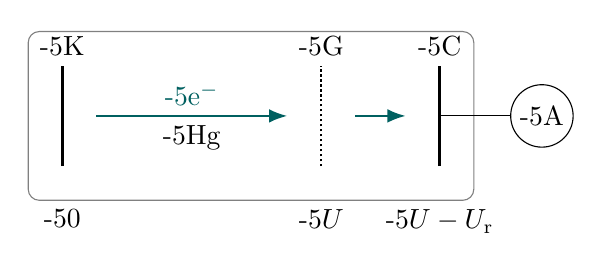
\begin{tikzpicture}[scale=.94,>=Latex,beam/.style={teal!75!black,thick,->}]
    \label{franck-hertz-tube}
    \def\gridX{3.5} \def\collectorX{5.1} \def\plate{.68} \def\wall{.46}
    \draw[rounded corners,black!50] (-\wall,-\plate-\wall) rectangle (\collectorX+\wall,\plate+\wall);
    \foreach \pos/\name/\potential in {0/K/0,\gridX/G/U,\collectorX/C/{U-U_{\retarding}}}{
        \node[above] at (\pos,\plate) {$\mathrm{\name}$};
        \node[below] at (\pos,-\plate-\wall) {$\potential$};
    }
    \draw[very thick] (0,-\plate) -- (0,\plate);
    \draw[thick,densely dotted] (\gridX,-\plate) -- (\gridX,\plate);
    \draw[very thick] (\collectorX,-\plate) -- (\collectorX,\plate);
    \draw[beam] (\wall,0) -- node[above] {$\electron^-$} (\gridX-\wall,0);
    \node[below] at (\gridX/2,0) {$\mathrm{Hg}$};
    \draw[beam] (\gridX+\wall,0) -- (\collectorX-\wall,0);
    \node[draw,circle,inner sep=2pt] (meter) at (\collectorX+3*\wall,0) {A};
    \draw (\collectorX,0) -- (meter.west);
\end{tikzpicture}

% 第 1 章
\standaloneconfig{border=3pt}
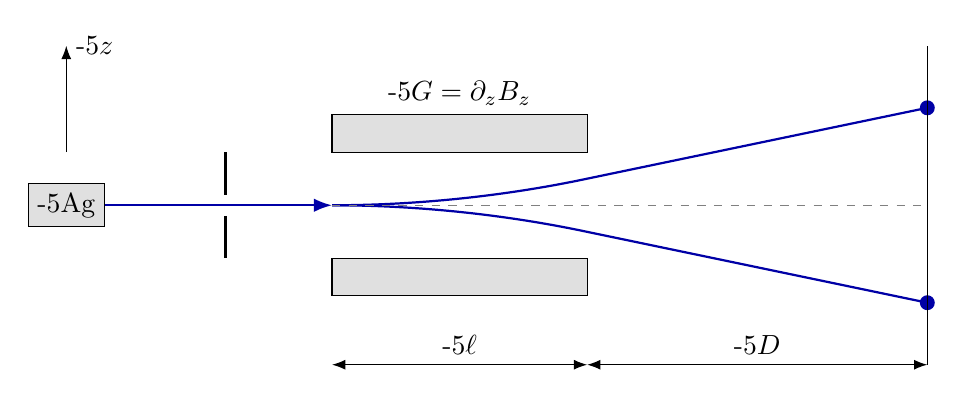
\begin{tikzpicture}[scale=1.35,>=Latex,beam/.style={blue!65!black,thick},hardware/.style={draw,fill=black!12}]
    \label{sg-beam}
    \def\slitX{-1.0} \def\ovenX{-2.5} \def\gap{0.10}
    \def\magLength{2.4} \def\drift{3.2} \def\exitHeight{0.25}
    \def\poleGap{0.5} \def\poleHeight{0.85} \def\dimensionY{-1.5}
    \pgfmathsetmacro{\screenX}{\magLength+\drift}
    \pgfmathsetmacro{\spot}{\exitHeight*(1+2*\drift/\magLength)}
    \node[hardware] (oven) at (\ovenX,0) {Ag};
    \draw[beam,->] (oven.east) -- (0,0);
    \foreach \side in {-1,1}{
        \draw[very thick] (\slitX,\side*\gap) -- (\slitX,\side*\poleGap);
        \draw[hardware] (0,\side*\poleGap) rectangle (\magLength,\side*\poleHeight);
        \draw[beam] (0,0) parabola (\magLength,\side*\exitHeight) -- (\screenX,\side*\spot);
        \fill[blue!65!black] (\screenX,\side*\spot) circle (2pt);
    }
    \draw (\screenX,\dimensionY) -- (\screenX,-\dimensionY);
    \draw[dashed,gray] (0,0) -- (\screenX,0);
    \node[above] at (\magLength/2,\poleHeight) {$G = \partial_z B_z$};
    \draw[<->] (0,\dimensionY) -- node[above] {$\ell$} (\magLength,\dimensionY);
    \draw[<->] (\magLength,\dimensionY) -- node[above] {$D$} (\screenX,\dimensionY);
    \draw[->] (\ovenX,\poleGap) -- (\ovenX,-\dimensionY) node[right] {$z$};
\end{tikzpicture}

\standaloneconfig{border=0pt}
\begin{tikzpicture}[>=Latex,
    stage/.style={draw=ink,fill=ink!5,minimum width=1.3cm,minimum height=.68cm},
    beam/.style={blue!65!black,thick},
    empty port/.style={gray,dashed}, occupied port/.style={beam,->}]
    \label{sg-filters}
    % 两行分别实验，末级的百分数均以抵达该级的原子为分母。
    \node[stage] (za) at (0,2.7) {$z$ 筛选};
    \node[stage] (finala) at (6.4,3.22) {$z$ 分析};
    \node[stage] (zb) at (0,0) {$z$ 筛选};
    \node[stage] (xb) at (3.2,.52) {$x$ 筛选};
    \node[stage] (finalb) at (6.4,1.04) {$z$ 分析};
    \foreach \stage/\panel in {za/a,zb/b}{
        \draw[beam,->] ($(\stage.west)+(-.9,0)$) node[left,text=black] {(\panel)}
            -- (\stage.west);
    }
    \foreach \src/\axis/\dst in {za/z/finala,zb/z/xb,xb/x/finalb}{
        \draw[beam,->] ($(\src.east)+(0,.12)$) -- ++(.62,.4)
            -- node[above,text=black] {$\ket{+\axis}$} (\dst.west);
        \draw[beam] ($(\src.east)+(0,-.12)$) -- ++(.62,-.4)
            -- ++(.65,0) coordinate (stop);
        \node[below] at ($(stop)+(-.32,0)$) {$-\axis$};
        \draw[black,very thick] ($(stop)+(0,-.13)$) -- ($(stop)+(0,.13)$);
    }
    \foreach \src/\upper/\lower/\lowerstyle in
        {finala/100/0/empty port,finalb/50/50/occupied port}{
        \draw[beam,->] ($(\src.east)+(0,.12)$) -- ++(.62,.4) -- ++(.46,0)
            node[right,text=black] {$+z\quad\upper\%$};
        \draw[\lowerstyle] ($(\src.east)+(0,-.12)$) -- ++(.62,-.4) -- ++(.46,0)
            node[right,text=black] {$-z\quad\lower\%$};
    }
\end{tikzpicture}

\begin{tikzpicture}[x=1cm,y=1cm, >=stealth]
    \label{spin-angle-readout}
    \begin{scope}[shift={(1.15,0)}]
        \draw[gray!60] (0,0) circle (1.25);
        \draw[->] (-1.4,0)--(1.6,0) node[right] {$x$};
        \draw[->] (0,-1.4)--(0,1.55) node[above] {$z$};
        \draw[->,very thick,blue!65!black] (0,0)--(35:1.25) node[above right] {$\bm n$};
        \draw (90:.52) arc (90:35:.52);
        \node at (63:.76) {$\gamma$};
        \node[below] at (0,-1.55) {分析器在 $xz$ 平面内转动};
    \end{scope}
    \begin{scope}[shift={(5.1,-1.25)},x=1.52cm,y=2.5cm]
        \draw[->] (0,0)--(3.52,0) node[right] {$\gamma/\unit{rad}$};
        \draw[->] (0,0)--(0,1.23) node[above] {$p$};
        \draw[densely dotted,gray] (0,.5)--(1.5708,.5)--(1.5708,0);
        \draw[very thick,blue!65!black,domain=0:3.14159,samples=48] plot (\x,{(1+cos(deg(\x)))/2});
        \draw[thick,dashed,black!70,domain=0:3.14159,samples=48] plot (\x,{(1-cos(deg(\x)))/2});
        \node[anchor=south west] at (.49,.95) {$+\bm n$};
        \node[anchor=south east] at (2.68,.95) {$-\bm n$};
        \node[left] at (0,1) {$1$};
        \node[left] at (0,.5) {$1/2$};
        \node[below] at (0,0) {$0$};
        \node[below] at (1.5708,0) {$\pi/2$};
        \node[below] at (3.14159,0) {$\pi$};
    \end{scope}
\end{tikzpicture}

% 相邻晶面 Bragg 散射的路程差。
\begin{tikzpicture}[>=Latex,
    ray/.style={ink,thick,postaction={decorate},decoration={
        markings,mark=at position .55 with {\arrow{Latex}}}},
    extra/.style={longwave,line width=1.5pt}]
    \label{bragg-path-difference}
    \def\braggAngle{34}
    \coordinate (lower) at (0,0);
    \coordinate (upper) at (0,1.75);
    \coordinate (incident) at ($(lower)+(180-\braggAngle:3.6)$);
    \coordinate (outgoing) at ($(lower)+(\braggAngle:3.6)$);
    % 上层散射点在下层两条传播方向上的垂足。
    \coordinate (left foot) at ($(lower)!(upper)!(incident)$);
    \coordinate (right foot) at ($(lower)!(upper)!(outgoing)$);

    \foreach \plane in {upper,lower}
        \draw[black!55] ($(\plane)+(-3.35,0)$) -- ($(\plane)+(3.35,0)$);
    \draw[ray] ($(upper)+(180-\braggAngle:2.6)$) node[above] {入射波} -- (upper);
    \draw[ray] (upper) -- ($(upper)+(\braggAngle:2.6)$) node[above] {散射波};
    \draw[ray] (incident) -- (lower);
    \draw[ray] (lower) -- (outgoing);

    \draw[black!65,dashed] (left foot) -- (upper) -- (right foot);
    \begin{scope}[shift={(left foot)},rotate=-\braggAngle]
        \draw[black!65] (.12,0) -- (.12,.12) -- (0,.12);
    \end{scope}
    \begin{scope}[shift={(right foot)},rotate=\braggAngle]
        \draw[black!65] (-.12,0) -- (-.12,.12) -- (0,.12);
    \end{scope}
    \draw[extra] (left foot) -- node[pos=.26,below left,inner sep=1.5pt] {$d\sin\theta$} (lower);
    \draw[extra] (lower) -- node[pos=.74,below right,inner sep=1.5pt] {$d\sin\theta$} (right foot);
    \draw[<->,black!75] (lower) -- node[midway,right,inner sep=2pt] {$d$} (upper);
    \draw (upper) ++(180:.65) arc[start angle=180,end angle=180-\braggAngle,radius=.65];
    \path (upper) ++(180-\braggAngle/2:.89) node {$\theta$};
\end{tikzpicture}

% 两路径干涉仪，正负端口按相位零点标定。
\begin{tikzpicture}[>=Latex,
    beam/.style={draw=blue!65!black,thick},
    traveling/.style={beam,postaction={decorate},decoration={
        markings,mark=at position .53 with {\arrow{Latex}}}},
    mirror/.style={draw=ink,line width=1.6pt},
    splitter/.style={draw=teal!70!black,line width=1.6pt,dashed},
    detector/.style={draw=ink,rounded corners=1.5pt,fill=black!4,inner sep=3pt}]
    \label{two-path-interferometer}
    \coordinate (split) at (0,0);
    \coordinate (upper) at (0,1.85);
    \coordinate (lower) at (4.8,0);
    \coordinate (combine) at (4.8,1.85);
    \node[left] (input) at (-1.45,0) {入射};
    \node[detector] (plus) at (7,1.85) {$+$ 探测器};
    \node[detector] (minus) at (4.8,3.05) {$-$ 探测器};
    \node[detector,fill=teal!6] (phase) at (2.4,0) {移相 $\varphi$};
    \draw[traveling] (input.east) -- (split);
    \draw[traveling] (split) -- (upper);
    \draw[traveling] (upper) -- node[above] {路径 $a$} (combine);
    \draw[traveling] (split) -- (phase.west);
    \draw[traveling] (phase.east) -- (lower);
    \draw[traveling] (lower) -- (combine);
    \node[below=1mm] at (phase.south) {路径 $b$};
    \draw[beam,->] (combine) -- (plus.west);
    \draw[beam,->] (combine) -- (minus.south);
    \foreach \optic in {split,combine}
        \draw[splitter] ($(\optic)+(-.24,-.24)$) -- ($(\optic)+(.24,.24)$);
    \foreach \optic/\back in {upper/1,lower/-1}{
        \begin{scope}[shift={(\optic)},rotate=45]
            \foreach \s in {-.30,-.18,-.06,.06,.18,.30}
                \draw[ink,thin] (\s,0) -- ++(.06,.09*\back);
        \end{scope}
        \draw[mirror] ($(\optic)+(-.24,-.24)$) -- ($(\optic)+(.24,.24)$);
    }
    \node[below left] at (split) {分束器};
    \node[below right] at (combine) {合束器};
\end{tikzpicture}

% 第 3 章
\standaloneconfig{border=5pt}
% 同一右手坐标系的正交投影。球面、赤道用纸面坐标，态和旋转轴用 xyz 坐标。
\tikzset{
    bloch coordinates/.style={x={(-.8cm,-.3cm)},y={(.6cm,-.4cm)},z={(0cm,.866025cm)}},
    bloch state/.style={curve,line width=1.35pt,-{Latex[length=2.2mm]}},
    bloch orbit/.style={curve,thick,postaction={decorate},
        decoration={markings,mark=at position .55 with {\arrow{Stealth[length=1.8mm]}}}},
    bloch rotation axis/.style={longwave,thick,densely dashed,-{Stealth[length=1.9mm]}}
}
\newcommand{\blochSphere}{%
    \draw[ink!40] (0,0) circle (1);
    \draw[ink!30,densely dashed] (-1,0) arc[start angle=180,end angle=0,x radius=1,y radius=.5];
    \draw[ink!43] (-1,0) arc[start angle=180,end angle=360,x radius=1,y radius=.5];
    \begin{scope}[bloch coordinates]
        \foreach \tip in {(1.38,0,0),(0,1.46,0),(0,0,1.39)}
            \draw[ink!60,-{Stealth[length=1.1mm]}] (0,0,0) -- \tip;
    \end{scope}
}
\newcommand{\blochLabels}{%
    \begin{scope}[bloch coordinates,every node/.style={inner sep=1pt,text=ink}]
        \node[left] at (1.38,0,0) {$x$};
        \node[below right] at (0,1.46,0) {$y$};
        \node[above] at (0,0,1.39) {$z$};
    \end{scope}
}

\begin{tikzpicture}
    \label{spin-precession}
    \foreach \pos/\phase/\angletext/\prob in
        {0/0/0/1,3.65/90/{\pi/2}/{1/2},7.3/180/{\pi}/0}{
        \begin{scope}[shift={(\pos,0)}]
            \blochSphere
            \blochLabels
            \begin{scope}[bloch coordinates]
                \ifnum\phase>0
                    \draw[bloch orbit] plot[variable=\a,domain=0:\phase,samples=48]
                        ({cos(\a)},{sin(\a)},0);
                \fi
                \draw[bloch state] (0,0,0) -- ({cos(\phase)},{sin(\phase)},0);
            \end{scope}
            \node[below,align=center] at (0,-1.08)
                {$\omega_0t = \angletext$\\$P_{+x} = \prob$};
        \end{scope}
    }
\end{tikzpicture}

\begin{tikzpicture}
    \label{rabi-axes}
    \foreach \pos/\tilt/\detuning in {0/0/0,3.45/45/\Omega}{
        \begin{scope}[shift={(\pos,0)}]
            \blochSphere
            \blochLabels
            \begin{scope}[bloch coordinates]
                \draw[bloch rotation axis] (0,0,0) -- ({1.27*cos(\tilt)},0,{1.27*sin(\tilt)});
                % 绕 (cos a,0,sin a) 将南极转过半圈；终点是首个布居峰。
                \draw[bloch orbit] plot[variable=\b,domain=0:180,samples=64]
                    ({-sin(\tilt)*cos(\tilt)*(1-cos(\b))},
                     {cos(\tilt)*sin(\b)},{-sin(\tilt)^2-cos(\tilt)^2*cos(\b)});
                \draw[bloch state] (0,0,0) -- ({-sin(2*\tilt)},0,{cos(2*\tilt)});
                \filldraw[draw=curve,fill=white] (0,0,-1) circle[radius=1.5pt];
            \end{scope}
            \node[below] at (0,-1.07) {$\Delta = \detuning$};
        \end{scope}
    }
\end{tikzpicture}

\begin{tikzpicture}[>=Latex,color=ink]
    \label{ramsey-sequence}
    \draw[->] (-1.6,0) -- (9.1,0) node[right] {$t$};
    \foreach \start/\angle in {.35/{\pi/2},5.05/{-\pi/2}}{
        \draw[draw=longwave,fill=longwave!12,thick] (\start,0) rectangle ++(.85,.49);
        \node[above] at (\start+.425,.49) {$R_y(\angle)$};
    }
    \draw[<->] (1.2,.26) -- node[fill=white,inner ysep=0pt] {自由演化 $T$} (5.05,.26);
    \node[above] at (-.9,0) {$\ket{+z}$};
    \draw[thick] (8,-.10) -- (8,.10) node[above] {沿 $z$ 测量};
    \foreach \pos/\stage in {1.2/第一脉冲后,4.65/等待结束,8/第二脉冲后}
        \node at (\pos,-.45) {\stage};
    \foreach \row/\phase/\sign/\xstate/\zstate/\prob in
        {-1.80/0/1/{+x}/{+z}/1,-3.68/\pi/-1/{-x}/{-z}/0}{
        \node[anchor=west] at (-1.7,\row) {$\Delta T = \phase$};
        \foreach \pos/\sx/\sz/\state in {1.2/1/0/{+x},4.65/\sign/0/\xstate,8/0/\sign/\zstate}{
            \begin{scope}[shift={(\pos,\row)},scale=.65]
                \blochSphere
                \begin{scope}[bloch coordinates]
                    \ifnum\sx=-1
                        \draw[bloch orbit] plot[variable=\a,domain=0:180,samples=40]
                            ({cos(\a)},{sin(\a)},0);
                    \fi
                    \draw[bloch state] (0,0,0) -- (\sx,0,\sz);
                \end{scope}
                \node[right] at (1.18,0) {$\ket{\state}$};
            \end{scope}
        }
        \node[right] at (9.65,\row) {$P_{+z} = \prob$};
    }
    \begin{scope}[shift={(1.2,-1.80)},scale=.65,font=\scriptsize]
        \blochLabels
    \end{scope}
\end{tikzpicture}

\begin{tikzpicture}[>=Latex,color=ink]
    \label{ammonia-inversion}
    \begin{scope}[x=1.5cm]
        \draw[->] (-2.95,0) -- (2.92,0) node[right] {$q$};
        \draw[->] (-2.95,0) -- (-2.95,2.95) node[above] {能量};
        \foreach \q/\energy in {-1.72/.25,0/2.05,1.72/.25}
            \draw[ink!42,densely dotted] (\q,-.32) -- (\q,\energy);
        \node[below right,inner sep=1pt] at (0,0) {$0$};
        \draw[very thick,ink] plot[variable=\q,domain=-2.55:2.55,samples=101]
            (\q,{.25+1.8*((\q/1.72)^2-1)^2});
        \node[above] at (0,2.05) {势垒顶 $V(0)$};
        \draw[curve,thick] (-2.12,.72) -- (2.12,.72);
        \draw[shortwave,thick,dashed] (-2.25,1.16) -- (2.25,1.16);
        \draw[<->] (2.57,.72) -- (2.57,1.16);
        \node[right] at (2.60,.94) {$2J$};
        \foreach \level/\value/\parity in {.72/{E_+=E_0-J}/对称,1.16/{E_-=E_0+J}/反对称}
            \node[right] at (3.22,\level) {$\value$（\parity）};
    \end{scope}
    % 氢三角形的中心是局部原点。整体绕 Ha 与中心的连线转半圈，N 换向，Hb、Hc 换位。
    \draw[ink!35] (4.12,-.52) -- (4.12,-2.55);
    \foreach \center/\heightN/\upperH/\lowerH/\showaxis/\description in {
        -2.58/-.68/b/c/1/{左阱 $\ket{\leftLabel}$},
        0/0/b/c/0/{四核共面},
        2.58/.68/b/c/0/{右阱 $\ket{\rightLabel}$},
        5.98/.68/c/b/1/{左阱构型整体转 $180^\circ$}}{
        \begin{scope}[shift={(\center,-1.43)}]
            \coordinate (N) at (0,\heightN);
            \coordinate (Ha) at (.96,0);
            \coordinate (Hupper) at (-.48,.45);
            \coordinate (Hlower) at (-.48,-.45);
            \filldraw[fill=ink!6,draw=ink!45,densely dashed] (Ha)--(Hupper)--(Hlower)--cycle;
            \foreach \atom in {Ha,Hupper,Hlower} \draw[ink,semithick] (N) -- (\atom);
            \ifnum\showaxis=1
                \draw[longwave,thick,dash dot] (-1.00,0) -- (1.25,0);
                \fill[longwave] (0,0) circle[radius=1.3pt];
            \fi
            \foreach \atom/\tag in {Ha/a,Hupper/\upperH,Hlower/\lowerH}
                \node[fill=white,inner sep=.5pt] at (\atom) {$\mathrm{H_{\tag}}$};
            \node[fill=white,inner sep=.7pt,text=curve] at (N) {$\mathrm N$};
            \node[below] at (0,-.86) {\description};
        \end{scope}
    }
\end{tikzpicture}

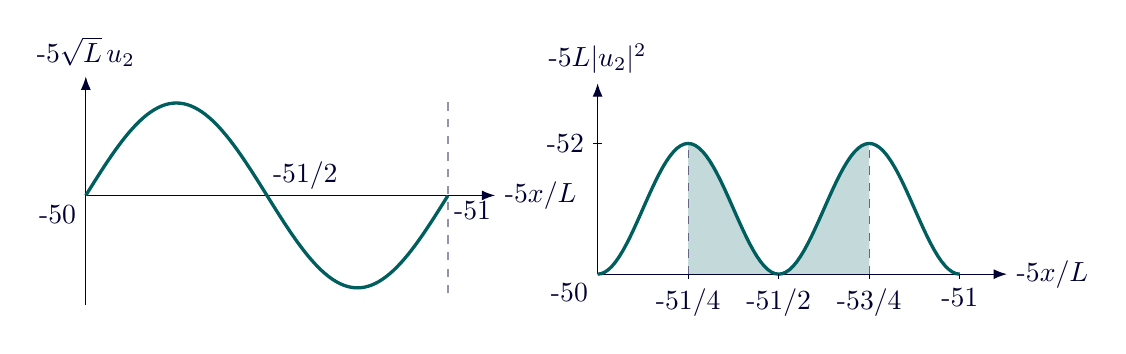
\begin{tikzpicture}[>=Latex,color=ink,x=4.6cm,y=.83cm]
    \label{well-detection}
    \begin{scope}
        \draw[->] (0,0) -- (1.13,0) node[right] {$x/L$};
        \draw[->] (0,-1.68) -- (0,1.82) node[above] {$\sqrt L\,u_2$};
        \draw[ink!42,dashed] (1,-1.50) -- (1,1.50);
        \draw[curve,very thick,domain=0:1,samples=101] plot (\x,{sqrt(2)*sin(360*\x)});
        \node[below left] at (0,0) {$0$};
        \node[above right,inner sep=2pt] at (.5,0) {$1/2$};
        \node[below right,inner sep=2pt] at (1,0) {$1$};
    \end{scope}
    \begin{scope}[xshift=6.5cm,yshift=-1.00cm]
        \fill[curve!23] (.25,0) -- plot[domain=.25:.75,samples=71] (\x,{2*sin(360*\x)^2}) -- (.75,0) -- cycle;
        \draw[ink!60,dashed] (.25,0) -- (.25,2) (.75,0) -- (.75,2);
        \draw[->] (0,0) -- (1.13,0) node[right] {$x/L$};
        \draw[->] (0,0) -- (0,2.92) node[above] {$L|u_2|^2$};
        \draw[curve,very thick,domain=0:1,samples=101] plot (\x,{2*sin(360*\x)^2});
        \draw (-.012,2) -- (.012,2) node[left=3pt] {$2$};
        \node[below left] at (0,0) {$0$};
        \foreach \x/\ticktext in {.25/{1/4},.5/{1/2},.75/{3/4},1/{1}}{
            \draw (\x,0) -- (\x,-.07) node[below] {$\ticktext$};
        }
    \end{scope}
\end{tikzpicture}

% 有限深方阱，z_0=3。z=ka 的两个根分别满足 z tan z=κa 和 -z cot z=κa。
\begin{tikzpicture}[scale=.85,>=Latex]
    \label{finite-well-parity}
    \def\zeven{1.17012095}
    \def\zodd{2.27886266}
    \pgfmathsetmacro{\decayeven}{sqrt(9-\zeven^2)}
    \pgfmathsetmacro{\decayodd}{sqrt(9-\zodd^2)}
    \begin{scope}[x=1.08cm,y=2.2cm]
        \draw[->] (-2.22,-1.12) -- (-2.22,.18) node[above] {$E/V_0$};
        \draw[->] (-2.22,-1.12) -- (2.25,-1.12) node[right] {$x/a$};
        \foreach \x in {-1,0,1}
            \draw (\x,-1.12) -- ++(0,-.035) node[below] {$\x$};
        \foreach \y in {-1,0}
            \draw (-2.22,\y) -- ++(-.06,0) node[left] {$\y$};
        \draw[very thick,ink] (-2.15,0) -- (-1,0) -- (-1,-1) -- (1,-1) -- (1,0) -- (2.15,0);
        \draw[thick,curve] (-1,{-(\decayeven/3)^2}) -- (1,{-(\decayeven/3)^2}) node[right] {偶态};
        \draw[thick,dashed,shortwave] (-1,{-(\decayodd/3)^2}) -- (1,{-(\decayodd/3)^2}) node[right] {奇态};
    \end{scope}
    \begin{scope}[xshift=6.95cm,yshift=-1.16cm,x=1.08cm,y=1.12cm]
        \draw[->] (-2.22,-1.16) -- (-2.22,1.19) node[above] {$u/\max\abs{u}$};
        \draw[->] (-2.22,-1.16) -- (2.25,-1.16) node[right] {$x/a$};
        \foreach \x in {-1,0,1}
            \draw (\x,-1.16) -- ++(0,-.065) node[below] {$\x$};
        \foreach \y in {-1,0,1}
            \draw (-2.22,\y) -- ++(-.06,0) node[left] {$\y$};
        \draw[black!35] (-2.15,0) -- (2.15,0);
        \foreach \x in {-1,1} \draw[densely dotted,black!50] (\x,-1.11) -- (\x,1.1);
        \draw[very thick,curve,samples=51,domain=-1:1] plot (\x,{cos(deg(\zeven*\x))});
        \draw[thick,dashed,shortwave,samples=51,domain=-1:1] plot (\x,{sin(deg(\zodd*\x))});
        \foreach \side in {-1,1}{
            \draw[very thick,curve,samples=28,domain=1:2.15]
                plot ({\side*\x},{cos(deg(\zeven))*exp(-\decayeven*(\x-1))});
            \draw[thick,dashed,shortwave,samples=28,domain=1:2.15]
                plot ({\side*\x},{\side*sin(deg(\zodd))*exp(-\decayodd*(\x-1))});
        }
    \end{scope}
\end{tikzpicture}

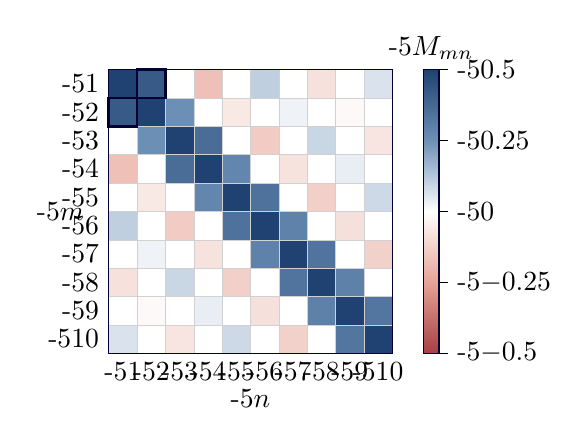
\begin{tikzpicture}[x=.36cm,y=-.36cm,/pgfplots/colormap name=matrix signed]
    \label{half-box-projector}
    \foreach \row in {1,...,10}{
        \foreach \column in {1,...,10}{
            % 半区间上对两个归一化正弦函数的乘积积分。
            \ifnum\row=\column\relax
                \def\matrixvalue{0.5}
            \else
                \pgfmathsetmacro{\matrixvalue}{
                    (sin(90*(\row-\column))/(\row-\column)
                    - sin(90*(\row+\column))/(\row+\column))/pi}
            \fi
            \pgfmathsetmacro{\colormapvalue}{1000*(\matrixvalue+0.5)}
            \pgfplotscolormapdefinemappedcolor{\colormapvalue}
            \filldraw[matrix cell,fill=mapped color]
                (\column-1,\row-1) rectangle (\column,\row);
        }
        \node[left] at (0,\row-.5) {$\row$};
        \node[below] at (\row-.5,10) {$\row$};
    }
    \draw[ink] (0,0) rectangle (10,10);
    \draw[ink,line width=.95pt] (1,0) rectangle (2,1) (0,1) rectangle (1,2);
    \node at (-1.7,5) {$m$};
    \node at (5,11.6) {$n$};
    \shade[shading=matrix signed] (11.1,10) rectangle (11.65,0);
    \draw[ink] (11.1,0) rectangle (11.65,10);
    \node[above] at (11.375,0) {$M_{mn}$};
    \foreach \tick in {-0.5,-0.25,0,0.25,0.5}{
        \draw (11.65,{5-10*\tick}) -- (11.95,{5-10*\tick})
            node[right] {$\tick$};
    }
\end{tikzpicture}

% 第 4 章
\standaloneconfig{border=4pt}
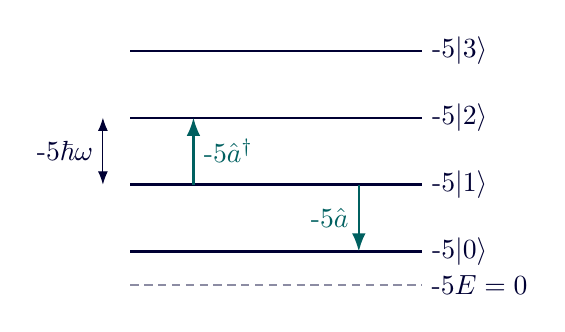
\begin{tikzpicture}[>=Latex,color=ink,level/.style={ink,thick},signal/.style={teal!75!black,thick},guide/.style={ink!45,densely dashed}]
    \label{oscillator-ladder}
\def\span{3.7} \def\step{.85} \def\inset{.8}
\foreach \n in {0,...,3}{
    \draw[level] (0,{(\n+.5)*\step}) -- (\span,{(\n+.5)*\step}) node[right] {$\ket{\n}$};
}
\draw[guide] (0,0) -- (\span,0) node[right,ink] {$E = 0$};
\draw[<->] (-.35,1.5*\step) -- node[left] {$\hbar\omega$} (-.35,2.5*\step);
\draw[signal,->] (\inset,1.5*\step) -- node[right] {$\op{a}\adjoint$} (\inset,2.5*\step);
\draw[signal,->] (\span-\inset,1.5*\step) -- node[left] {$\op{a}$} (\span-\inset,.5*\step);
\end{tikzpicture}

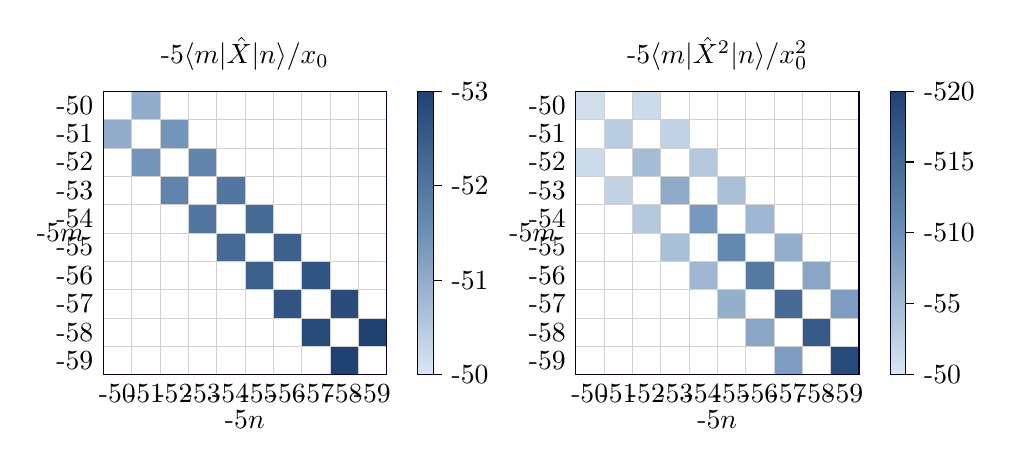
\begin{tikzpicture}[x=.36cm,y=-.36cm,/pgfplots/colormap name=matrix sequential]
    \label{oscillator-position-matrices}
    \foreach \power/\limit/\ticks/\offset in {1/3/{0,1,2,3}/0cm,2/20/{0,5,10,15,20}/6cm}{
        \begin{scope}[xshift=\offset]
            \foreach \row in {0,...,9}{
                \foreach \column in {0,...,9}{
                    \ifnum\power=1
                        \pgfmathsetmacro{\matrixvalue}{
                            ifthenelse(abs(\row-\column)==1,sqrt(max(\row,\column)),0)}
                    \else
                        % 取全空间的 X^2 矩阵元，再截取所画的行与列。
                        \pgfmathsetmacro{\higher}{max(\row,\column)}
                        \pgfmathsetmacro{\matrixvalue}{
                            ifthenelse(\row==\column,2*\column+1,
                            ifthenelse(abs(\row-\column)==2,sqrt(\higher*(\higher-1)),0))}
                    \fi
                    \pgfmathsetmacro{\colormapvalue}{1000*(\matrixvalue/\limit)}
                    \pgfplotscolormapdefinemappedcolor{\colormapvalue}
                    \ifdim\matrixvalue pt=0pt\relax \colorlet{mapped color}{white}\fi
                    \filldraw[matrix cell,fill=mapped color]
                        (\column,\row) rectangle ++(1,1);
                }
                \node[left] at (0,\row+.5) {$\row$};
                \node[below] at (\row+.5,10) {$\row$};
            }
            \draw[ink] (0,0) rectangle (10,10);
            \node at (-1.5,5) {$m$};
            \node at (5,11.6) {$n$};
            \ifnum\power=1
                \node[above] at (5,-.4) {$\mel{m}{\op X}{n}/x_0$};
            \else
                \node[above] at (5,-.4) {$\mel{m}{\op X^2}{n}/x_0^2$};
            \fi
            \shade[bottom color=matrixpale,top color=matrixnavy,middle color=matrixblue]
                (11.1,10) rectangle (11.65,0);
            \draw[ink] (11.1,0) rectangle (11.65,10);
            \foreach \tick in \ticks {
                \draw (11.65,{10*(1-\tick/\limit)}) -- (11.95,{10*(1-\tick/\limit)})
                    node[right] {$\tick$};
            }
        \end{scope}
    }
\end{tikzpicture}

% 第 5 章
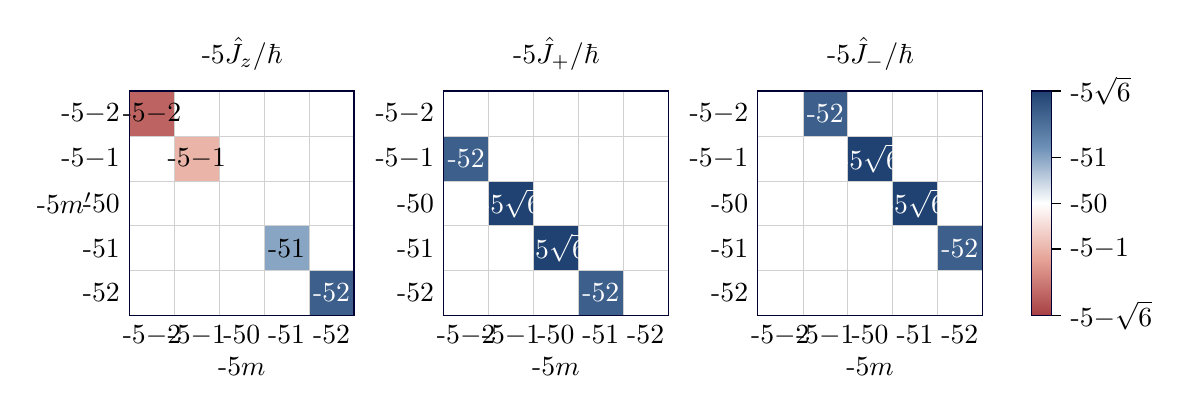
\begin{tikzpicture}[x=.57cm,y=-.57cm,/pgfplots/colormap name=matrix signed]
    \label{angular-momentum-matrices}
    \foreach \matrixstep/\component/\offset in {0/z/0,1/+/7,-1/-/14}{
        \begin{scope}[shift={(\offset,0)}]
            \foreach \gridline in {1,...,4}{
                \draw[black!18,line width=.2pt]
                    (\gridline,0) -- (\gridline,5) (0,\gridline) -- (5,\gridline);
            }
            \foreach \inputm in {-2,...,2}{
                \pgfmathtruncatemacro{\outputm}{\inputm+\matrixstep}
                \ifnum\matrixstep=0
                    \let\matrixvalue\inputm
                    \let\entry\inputm
                \else
                    \pgfmathtruncatemacro{\radicand}{6-(\inputm)*(\outputm)}
                    \pgfmathsetmacro{\matrixvalue}{sqrt(\radicand)}
                    \ifnum\radicand=4
                        \def\entry{2}
                    \else
                        \def\entry{\sqrt{\radicand}}
                    \fi
                \fi
                \ifdim\matrixvalue pt=0pt\relax
                \else
                    \pgfmathsetmacro{\colormapvalue}{500*(1+\matrixvalue/sqrt(6))}
                    \pgfplotscolormapdefinemappedcolor{\colormapvalue}
                    \filldraw[matrix cell,fill=mapped color]
                        (\inputm+2,\outputm+2) rectangle ++(1,1);
                    \def\textcolorname{black}
                    \ifdim\matrixvalue pt>1.5pt\relax \def\textcolorname{white}\fi
                    \node[text=\textcolorname] at (\inputm+2.5,\outputm+2.5) {$\entry$};
                \fi
            }
            \foreach \state in {-2,...,2}{
                \node[left] at (0,\state+2.5) {$\state$};
                \node[below] at (\state+2.5,5) {$\state$};
            }
            \draw[ink] (0,0) rectangle (5,5);
            \node[above] at (2.5,-.25) {$\op{J}_{\component}/\hbar$};
            \node at (2.5,6.15) {$m$};
        \end{scope}
    }
    \node at (-1.45,2.5) {$m'$};
    \shade[shading=matrix signed] (20.1,5) rectangle (20.55,0);
    \draw[ink] (20.1,0) rectangle (20.55,5);
    \foreach \level/\tick in {{-sqrt(6)}/{-\sqrt{6}},-1/-1,0/0,1/1,{sqrt(6)}/{\sqrt{6}}}{
        \pgfmathsetmacro{\tickrow}{2.5*(1-(\level)/sqrt(6))}
        \draw (20.55,\tickrow) -- (20.75,\tickrow) node[right] {$\tick$};
    }
\end{tikzpicture}

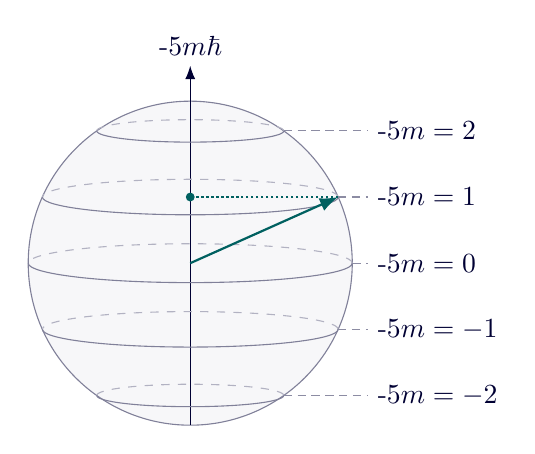
\begin{tikzpicture}[>=Latex,color=ink,level/.style={ink,thick},signal/.style={teal!75!black,thick},guide/.style={ink!45,densely dashed}]
    \label{angular-projection}
\def\ell{2} \def\momentumScale{.84} \def\tilt{.12}
\pgfmathsetmacro{\radius}{sqrt(\ell*(\ell+1))*\momentumScale}
\filldraw[fill=ink!3,draw=ink!50] (0,0) circle (\radius);
\draw[->] (0,-\radius) -- (0,\radius+.45) node[above] {$m\hbar$};
\foreach \m in {-2,...,2}{
    \pgfmathsetmacro{\ring}{sqrt(\radius^2-(\momentumScale*\m)^2)}
    \draw[ink!30,dashed] (\ring,\momentumScale*\m) arc[start angle=0,end angle=180,x radius=\ring,y radius=\ring*\tilt];
    \draw[ink!50] (-\ring,\momentumScale*\m) arc[start angle=180,end angle=360,x radius=\ring,y radius=\ring*\tilt];
    \draw[guide] (\ring,\momentumScale*\m) -- (\radius+.2,\momentumScale*\m) node[right,ink] {$m = \m$};
}
\pgfmathsetmacro{\reach}{sqrt(\radius^2-\momentumScale^2)}
\draw[signal,->] (0,0) -- (\reach,\momentumScale);
\draw[signal,densely dotted] (\reach,\momentumScale) -- (0,\momentumScale);
\fill[teal!75!black] (0,\momentumScale) circle (1.6pt);
\end{tikzpicture}

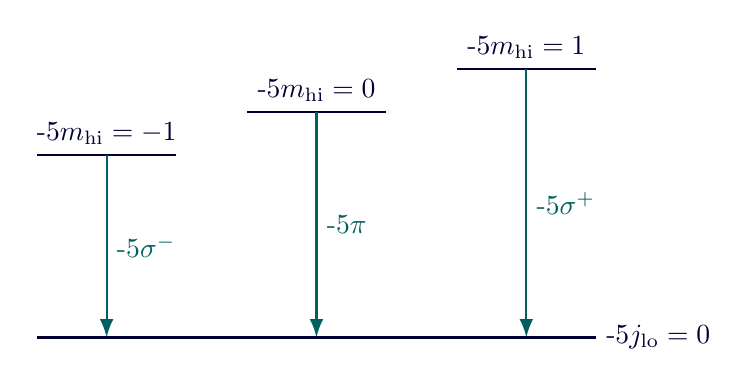
\begin{tikzpicture}[scale=1.3,>=Latex,color=ink,level/.style={ink,thick},signal/.style={teal!75!black,thick},guide/.style={ink!45,densely dashed}]
    \label{zeeman-triplet}
\def\col{2.05} \def\halfwidth{.68} \def\excited{2.2} \def\split{.42}
\draw[level] (-\col-\halfwidth,0) -- (\col+\halfwidth,0) node[right] {$j_\lo = 0$};
\foreach \m/\pol in {-1/\sigma^-,0/\pi,1/\sigma^+}{
    \draw[level] (\m*\col-\halfwidth,\excited+\m*\split) -- ++(2*\halfwidth,0) node[midway,above] {$m_\hi = \m$};
    \draw[signal,->] (\m*\col,\excited+\m*\split) -- node[right] {$\pol$} (\m*\col,0);
}
\end{tikzpicture}

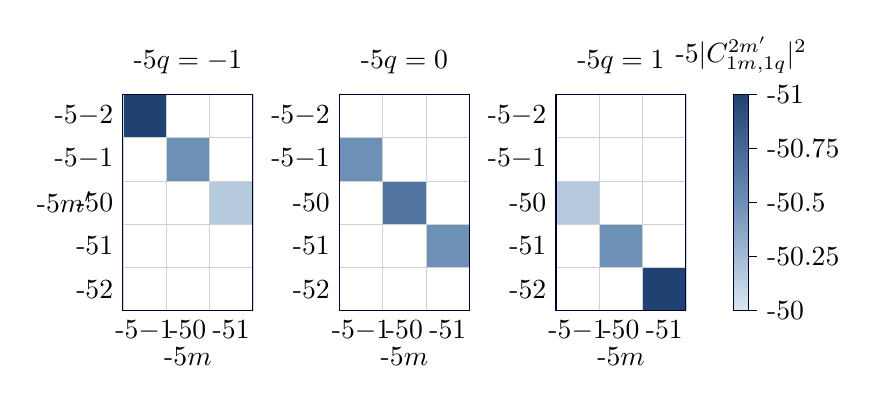
\begin{tikzpicture}[x=.55cm,y=-.55cm,/pgfplots/colormap name=matrix sequential]
    \label{dipole-selection-matrices}
    \foreach \component/\offset in {-1/0,0/5,1/10}{
        \begin{scope}[shift={(\offset,0)}]
            \foreach \initialm in {-1,0,1}{
                \foreach \finalm in {-2,...,2}{
                    % C^{2,m+q}_{1m,1q} 的模平方。
                    \pgfmathsetmacro{\strength}{
                        ifthenelse(\finalm==\initialm+\component,
                        ifthenelse(\component==0,(4-(\initialm)^2)/6,
                        (\initialm*\component+2)*(\initialm*\component+3)/12),0)}
                    \pgfmathsetmacro{\colormapvalue}{1000*\strength}
                    \pgfplotscolormapdefinemappedcolor{\colormapvalue}
                    \ifdim\strength pt=0pt\relax \colorlet{mapped color}{white}\fi
                    \filldraw[matrix cell,fill=mapped color]
                        (\initialm+1,\finalm+2) rectangle ++(1,1);
                }
                \node[below] at (\initialm+1.5,5) {$\initialm$};
            }
            \foreach \finalm in {-2,...,2}
                \node[left] at (0,\finalm+2.5) {$\finalm$};
            \draw[ink] (0,0) rectangle (3,5);
            \node[above] at (1.5,-.25) {$q = \component$};
            \node at (1.5,6.05) {$m$};
        \end{scope}
    }
    \node at (-1.35,2.5) {$m'$};
    \shade[bottom color=matrixpale,top color=matrixnavy,middle color=matrixblue]
        (14.1,5) rectangle (14.45,0);
    \draw[ink] (14.1,0) rectangle (14.45,5);
    \node[above] at (14.275,-.25) {$\abs{C^{2m'}_{1m,1q}}^2$};
    \foreach \tick in {0,0.25,0.5,0.75,1}{
        \draw (14.45,{5*(1-\tick)}) -- (14.65,{5*(1-\tick)})
            node[right] {$\tick$};
    }
\end{tikzpicture}

% 第 6 章
\begin{tikzpicture}[>=Latex,color=ink,level/.style={ink,thick},signal/.style={teal!75!black,thick},guide/.style={ink!45,densely dashed}]
    \label{hydrogen-levels}
\def\binding{5.4} \def\column{1.45} \def\halfline{.52}
\foreach \ell/\orb in {0/s,1/p,2/d,3/f}{
    \node at (\ell*\column,.42) {$\mathrm{\orb}$};
    \foreach \n in {1,...,4}{\ifnum\n>\ell
        \draw[level] (\ell*\column-\halfline,-\binding/\n^2) -- ++(2*\halfline,0);
    \fi}
}
\draw[guide] (-\halfline,0) -- (3*\column+\halfline,0) node[right,ink] {$E = 0$};
\foreach \n/\offset in {1/0,2/0,3/-1.5,4/1.5}
    \node[left,yshift=\offset pt] at (-\halfline,-\binding/\n^2) {$n = \n$};
\def\finalN{2}
\foreach \n/\initialL/\finalL/\tag/\linecolor in {3/1/0/\upalpha/balmerAlpha,4/2/1/\upbeta/balmerBeta}{
    \draw[\linecolor,thick,->] (\initialL*\column,-\binding/\n^2) -- node[near end,above,sloped] {$\atomH_{\tag}$} (\finalL*\column,-\binding/\finalN^2);
}
\end{tikzpicture}

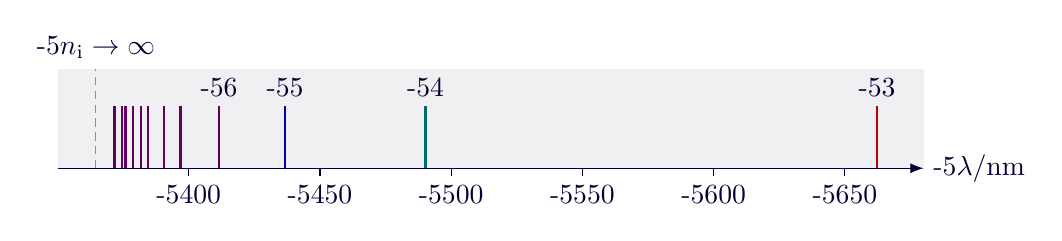
\begin{tikzpicture}[scale=1.1,>=Latex,color=ink,level/.style={ink,thick},signal/.style={teal!75!black,thick},guide/.style={ink!45,densely dashed}]
    \label{balmer-lines}
\def\rydberg{0.0109678} \def\start{350} \def\stop{680} \def\axiswidth{10}
\def\lineheight{.72} \def\stripheight{1.15}
\pgfmathdeclarefunction{pos}{1}{\pgfmathparse{(#1-\start)*\axiswidth/(\stop-\start)}}
\fill[ink!6] (0,0) rectangle (\axiswidth,\stripheight);
\foreach \n in {3,...,14}{
    \pgfmathsetmacro{\wave}{1/(\rydberg*(1/4-1/\n^2))}
    \colorlet{linecolor}{violet!75!black}
    \ifnum\n=3 \colorlet{linecolor}{balmerAlpha}\fi
    \ifnum\n=4 \colorlet{linecolor}{balmerBeta}\fi
    \ifnum\n=5 \colorlet{linecolor}{blue!70!black}\fi
    \draw[linecolor,thick] ({pos(\wave)},0) -- ++(0,\lineheight);
    \ifnum\n<7 \node[above] at ({pos(\wave)},\lineheight) {$\n$};\fi
}
\draw[guide] ({pos(4/\rydberg)},0) -- ++(0,\stripheight) node[above,ink] {$n_\initial \to \infty$};
\draw[->] (0,0) -- (\axiswidth,0) node[right] {$\lambda/\unit{nm}$};
\foreach \tick in {400,450,...,650}\draw ({pos(\tick)},0) -- ++(0,-.09) node[below] {$\tick$};
\end{tikzpicture}

% 第 8 章
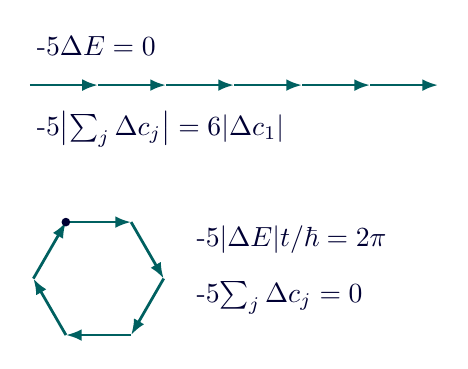
\begin{tikzpicture}[scale=1.2,color=ink,amplitude/.style={-{Latex[length=2mm]},line width=1pt,draw=amplitude}]
    \label{transition-phasors}
    \node[anchor=west] at (-.03,2.20) {$\Delta E = 0$};
    \foreach \step in {0,...,5}{
        \draw[amplitude] (.72*\step,1.79) -- ++(.72,0);
    }
    \node[anchor=west] at (-.03,1.32)
        {$\bigabs{\sum_j\Delta c_j} = 6\abs{\Delta c_1}$};

    \coordinate (start) at (.38,.34);
    \coordinate (tip) at (start);
    \foreach \angle in {0,-60,-120,-180,-240,-300}{
        \draw[amplitude] (tip) -- ++(\angle:.69) coordinate (tip);
    }
    \fill[ink] (start) circle (1.3pt);
    \node[anchor=west] at (1.66,.16) {$|\Delta E|t/\hbar = 2\pi$};
    \node[anchor=west] at (1.66,-.46) {$\sum_j\Delta c_j = 0$};
\end{tikzpicture}

% 第 9 章
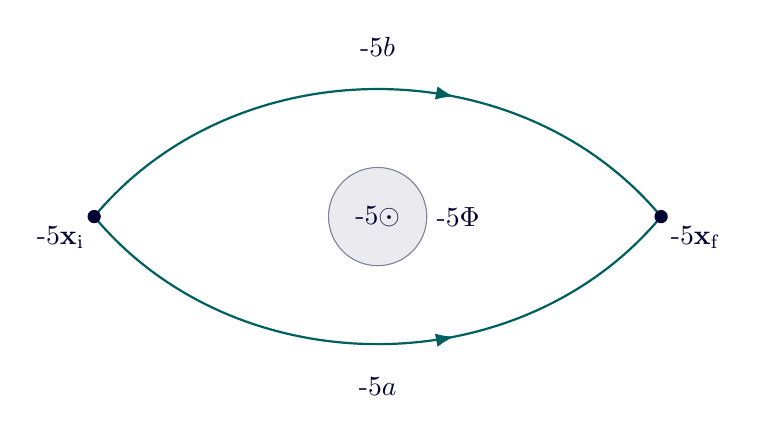
\begin{tikzpicture}[scale=1.2,>=Latex,color=ink,level/.style={ink,thick},signal/.style={teal!75!black,thick},guide/.style={ink!45,densely dashed}]
    \label{flux-paths}
\def\arm{3} \def\height{1.8} \def\core{.52}
\filldraw[draw=ink!50,fill=ink!8] (0,0) circle (\core);
\node at (0,0) {$\odot$}; \node[right] at (\core,0) {$\Phi$};
\foreach \side/\branch in {-1/a,1/b}{
    \draw[signal,postaction={decorate},decoration={markings,mark=at position .62 with {\arrow{Latex}}}]
    (-\arm,0) .. controls (-\arm/2,\side*\height) and (\arm/2,\side*\height) .. (\arm,0);
    \node at (0,\side*\height) {$\branch$};
}
\foreach \side/\point/\anchor in {-1/\initial/north east,1/\final/north west}{
    \fill (\side*\arm,0) circle (2pt) node[anchor=\anchor] {$\mathbf x_\point$};
}
\end{tikzpicture}

\standaloneconfig{border=0pt}
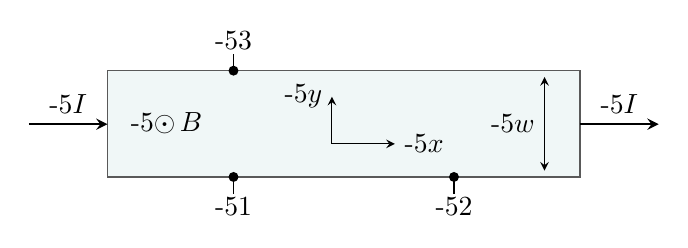
\begin{tikzpicture}[x=1cm,y=1cm,>=stealth]
    \label{hall-voltage}
    \filldraw[fill=teal!6,draw=black!65] (0,0) rectangle (6,1.35);
    \draw[->,thick] (-1,.67) -- (0,.67) node[midway,above] {$I$};
    \draw[->,thick] (6,.67) -- (7,.67) node[midway,above] {$I$};
    \foreach \x/\y/\dy/\lab in {1.6/0/-.38/1,4.4/0/-.38/2,1.6/1.35/.38/3}{
        \fill (\x,\y) circle (1.8pt);
        \draw (\x,\y) -- ++(0,\dy) node[fill=white,inner sep=1.5pt] {$\lab$};
    }
    \draw[<->] (5.55,.08) -- (5.55,1.27) node[midway,left] {$w$};
    \draw[->] (2.85,.42) -- (3.65,.42) node[right] {$x$};
    \draw[->] (2.85,.42) -- (2.85,1.02) node[left] {$y$};
    \node at (.75,.68) {$\odot \,B$};
\end{tikzpicture}

% 第 11 章
\standaloneconfig{border=3pt}
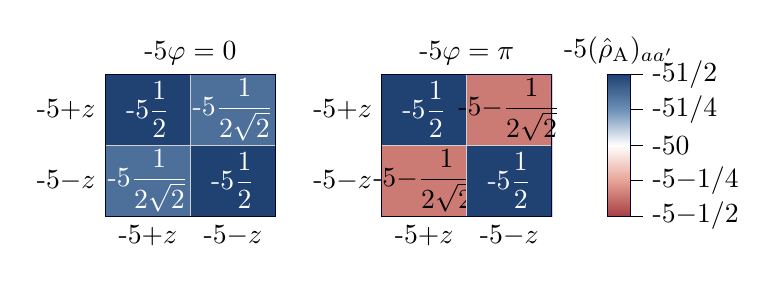
\begin{tikzpicture}[x=1.08cm,y=-.9cm,/pgfplots/colormap name=matrix signed]
    \label{reduced-spin-density-matrices}
    \foreach \relativeSign/\phase/\offset in {1/0/0,-1/\pi/3.25}{
        \begin{scope}[shift={(\offset,0)}]
            \foreach \row in {0,1}{
                \foreach \column in {0,1}{
                    \ifnum\row=\column
                        \def\matrixvalue{0.5}
                        \def\entry{\dfrac{1}{2}}
                    \else
                        \pgfmathsetmacro{\matrixvalue}{\relativeSign/(2*sqrt(2))}
                        \ifnum\relativeSign>0
                            \def\entry{\dfrac{1}{2\sqrt{2}}}
                        \else
                            \def\entry{-\dfrac{1}{2\sqrt{2}}}
                        \fi
                    \fi
                    \pgfmathsetmacro{\colormapvalue}{1000*(\matrixvalue+0.5)}
                    \pgfplotscolormapdefinemappedcolor{\colormapvalue}
                    \filldraw[matrix cell,fill=mapped color] (\column,\row) rectangle ++(1,1);
                    \def\textcolorname{black}
                    \ifdim\matrixvalue pt>0pt\relax \def\textcolorname{white}\fi
                    \node[text=\textcolorname] at (\column+.5,\row+.5) {$\entry$};
                }
            }
            \draw[ink] (0,0) rectangle (2,2);
            \node[left] at (0,.5) {$+z$};
            \node[left] at (0,1.5) {$-z$};
            \node[below] at (.5,2) {$+z$};
            \node[below] at (1.5,2) {$-z$};
            \node[above] at (1,0) {$\varphi = \phase$};
        \end{scope}
    }
    \shade[shading=matrix signed] (5.9,2) rectangle (6.18,0);
    \draw[ink] (5.9,0) rectangle (6.18,2);
    \node[above] at (6.04,0) {$(\op\rho_{\subsysA})_{aa'}$};
    \foreach \level/\tick in {-.5/{-1/2},-.25/{-1/4},0/0,.25/{1/4},.5/{1/2}}{
        \draw (6.18,{1-2*\level}) -- (6.32,{1-2*\level}) node[right] {$\tick$};
    }
\end{tikzpicture}

\definecolor{fringeblue}{HTML}{233782}
\begin{tikzpicture}
    \label{quantum-eraser-fringes}
    \begin{axis}[
        scale only axis,width=10cm,height=3.7cm,
        xmin=0,xmax=2,ymin=-.035,ymax=1.035,
        axis lines=left,axis line style={draw=ink,line width=.5pt},
        tick align=outside,tick style={draw=ink},
        xtick={0,.5,1,1.5,2},xticklabels={$0$,$1/2$,$1$,$3/2$,$2$},
        ytick={0,.25,.5,.75,1},
        xlabel={$\varphi/\pi$},ylabel={正端概率},
        ymajorgrids,major grid style={draw=black!13},
        domain=0:2,samples=101,
        legend columns=3,
        legend style={at={(.5,1.045)},anchor=south,draw=none,
            /tikz/every even column/.append style={column sep=6mm}},
    ]
        \addplot[fringeblue,line width=1pt] {(1+cos(180*x))/2};
        \addlegendentry{$\P(+ \mid D_+)$}
        \addplot[matrixbrick,line width=1pt,dashed] {(1-cos(180*x))/2};
        \addlegendentry{$\P(+ \mid D_-)$}
        \addplot[black!75,line width=.9pt,densely dotted,samples=2] {0.5};
        \addlegendentry{合并 $P_+$}
    \end{axis}
\end{tikzpicture}

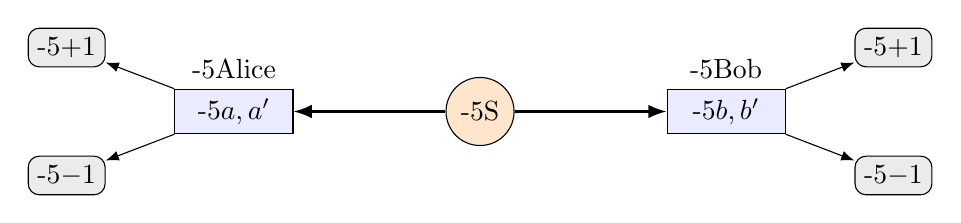
\begin{tikzpicture}[scale=1.25,>=Latex,station/.style={draw,fill=blue!8,minimum width=1.5cm},detector/.style={draw,rounded corners,fill=black!8}]
    \label{bell-pair}
    \def\arm{2.5} \def\readout{1.7} \def\split{0.65}
    \node[draw,circle,fill=orange!20] (source) at (0,0) {$\mathrm{S}$};
    \foreach \side/\name/\settings in {-1/Alice/{a,a'},1/Bob/{b,b'}}{
        \node[station,label=above:\name] (analyzer) at (\side*\arm,0) {$\settings$};
        \draw[->,thick] (source) -- (analyzer);
        \foreach \sign/\value in {1/+1,-1/-1}{
            \node[detector] (counter) at ({\side*(\arm+\readout)},\sign*\split) {$\value$};
            \draw[->] (analyzer) -- (counter);
        }
    }
\end{tikzpicture}

% 第 12 章
\standaloneconfig{border=4pt}
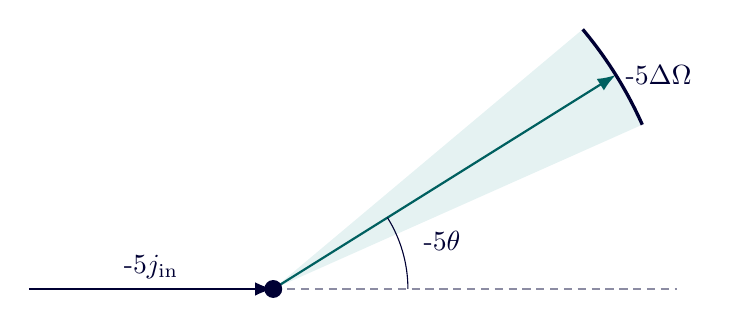
\begin{tikzpicture}[scale=1.35,>=Latex,color=ink,level/.style={ink,thick},signal/.style={teal!75!black,thick},guide/.style={ink!45,densely dashed}]
    \label{scattering-aperture}
\def\angleout{32} \def\aperture{8} \def\distance{3.8} \def\beamlength{2.3}
\fill[teal!10] (0,0) -- (\angleout-\aperture:\distance) arc[start angle=\angleout-\aperture,end angle=\angleout+\aperture,radius=\distance] -- cycle;
\draw[guide] (0,0) -- (\distance,0);
\draw[->,thick] (-\beamlength,0) -- node[above] {$j_{\rm in}$} (0,0);
\draw[signal,->] (0,0) -- (\angleout:\distance);
\draw[ink,very thick] (\angleout-\aperture:\distance) arc[start angle=\angleout-\aperture,end angle=\angleout+\aperture,radius=\distance];
\node[right] at (\angleout:\distance) {$\Delta\Omega$};
\draw (0:\distance/3) arc[start angle=0,end angle=\angleout,radius=\distance/3];
\node at (\angleout/2:\distance/2.3) {$\theta$}; \fill (0,0) circle (2.4pt);
\end{tikzpicture}

\standaloneconfig{border=0pt}
\begin{tikzpicture}[x=1.07cm,y=.75cm,>=stealth]
    \label{hard-sphere-nodes}
    \fill[black!8] (0,-1.10) rectangle (1,1.12);
    \draw[->] (-.15,0) -- (8.7,0) node[right] {$r/a$};
    \draw[->] (0,-1.2) -- (0,1.6) node[above] {$u_0$};
    \draw[black!65,dashed,thick] plot[domain=0:8.5,samples=100]
        (\x,{sin(45*\x)});
    \draw[teal!70!black,thick] plot[domain=1:8.5,samples=100]
        (\x,{sin(45*(\x-1))});
    \draw[black!50] (1,-1.1) -- (1,1.12);
    \foreach \tick in {1,4,5,8}
        \draw (\tick,.06) -- (\tick,-.06) node[below,fill=white,inner sep=1pt] {$\tick$};
    \node[anchor=west,inner sep=0pt] at (.95,1.68) {自由径向波};
    \draw[dashed,thick,black!65] (.2,1.68) -- (.85,1.68);
    \node[anchor=west,inner sep=0pt] at (4.5,1.68) {硬球外的径向波};
    \draw[teal!70!black,thick] (3.75,1.68) -- (4.4,1.68);
\end{tikzpicture}

% 第 13 章
\standaloneconfig{border=4pt}
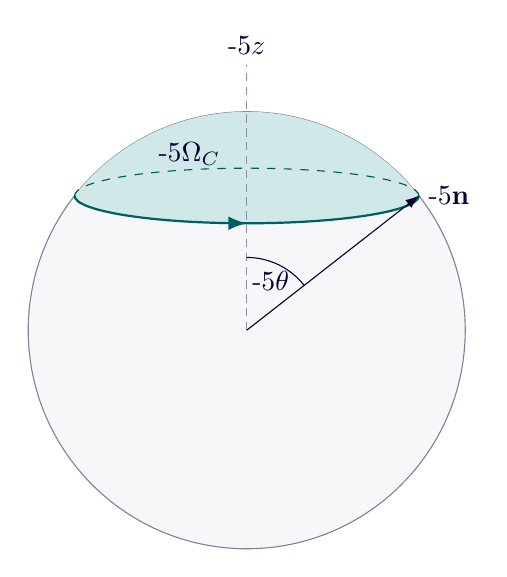
\begin{tikzpicture}[scale=1.5,>=Latex,color=ink,level/.style={ink,thick},signal/.style={teal!75!black,thick},guide/.style={ink!45,densely dashed}]
    \label{berry-cap}
\def\radius{1.85} \def\polar{52} \def\flatten{.16}
\pgfmathsetmacro{\ring}{\radius*sin(\polar)} \pgfmathsetmacro{\height}{\radius*cos(\polar)}
\draw[ink!50,fill=ink!3] (0,0) circle (\radius);
\fill[teal!18] (\ring,\height) arc[start angle=90-\polar,end angle=90+\polar,radius=\radius] arc[start angle=180,end angle=360,x radius=\ring,y radius=\ring*\flatten];
\draw[guide] (0,0) -- (0,\radius+.4) node[above,ink] {$z$};
\draw[teal!70!black,dashed] (\ring,\height) arc[start angle=0,end angle=180,x radius=\ring,y radius=\ring*\flatten];
\draw[signal,postaction={decorate},decoration={markings,mark=at position .5 with {\arrow{Latex}}}] (-\ring,\height) arc[start angle=180,end angle=360,x radius=\ring,y radius=\ring*\flatten];
\draw[->] (0,0) -- (\ring,\height) node[right] {$\mathbf n$};
\draw (90:\radius/3) arc[start angle=90,end angle=90-\polar,radius=\radius/3];
\node at (90-\polar/2:\radius/4) {$\theta$};
\node at (-\ring/3,{(\height+\radius)/2}) {$\Omega_C$};
\end{tikzpicture}

% 第 15 章
\begin{tikzpicture}[scale=1.25,>=Latex,level/.style={very thick,blue!20!black},
    guide/.style={densely dashed,black!45},shifted/.style={very thick,teal!75!black}]
    \label{hydrogen-fine-lamb}
    \def\column{3.5} \def\halfwidth{.96} \def\fineGap{2.2} \def\lambGap{.72}
    \pgfmathsetmacro{\lower}{-5*\fineGap/4}
    \pgfmathsetmacro{\upper}{-\fineGap/4}
    \foreach \col/\title in {0/Coulomb,1/Dirac,2/{Dirac + Lamb}}{
        \node[above] at (\col*\column,.48) {\textsf{\title}};
    }
    \draw[level] (-\halfwidth,0) -- node[above] {$n = 2$} (\halfwidth,0);
    \foreach \energy/\term in {\upper/{2\orbitalP_{3/2}},\lower/{2\orbitalS_{1/2},\,2\orbitalP_{1/2}}}{
        \draw[guide] (\halfwidth,0) -- (\column-\halfwidth,\energy);
        \draw[level] (\column-\halfwidth,\energy) -- node[above] {$\term$} (\column+\halfwidth,\energy);
        \draw[guide] (\column+\halfwidth,\energy) -- (2*\column-\halfwidth,\energy);
    }
    \draw[guide] (\column+\halfwidth,\lower) -- (2*\column-\halfwidth,\lower+\lambGap);
    \foreach \energy/\term/\style in {\upper/{2\orbitalP_{3/2}}/level,\lower/{2\orbitalP_{1/2}}/level,
        {\lower+\lambGap}/{2\orbitalS_{1/2}}/shifted}{
        \draw[\style] (2*\column-\halfwidth,\energy) -- node[above] {$\term$} (2*\column+\halfwidth,\energy);
    }
    \draw[<->] (2*\column+1.2*\halfwidth,\lower) -- node[right] {$h\nu_{\rm L}$}
        (2*\column+1.2*\halfwidth,\lower+\lambGap);
\end{tikzpicture}

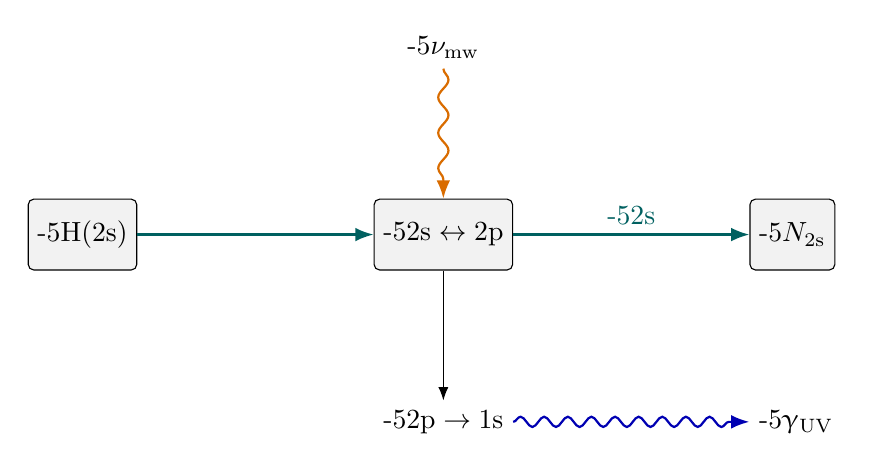
\begin{tikzpicture}[>=Latex,beam/.style={teal!75!black,thick,->},
    stage/.style={draw,rounded corners=2pt,fill=black!5,minimum height=9mm}]
    \label{lamb-readout}
    \def\drift{3} \def\driveGap{1.65}
    \node[stage] (source) {$\atomH(2\orbitalS)$};
    \node[stage,right=\drift cm of source] (drive) {$2\orbitalS \leftrightarrow 2\orbitalP$};
    \node[stage,right=\drift cm of drive] (detector) {$N_{2\orbitalS}$};
    \draw[beam] (source) -- (drive);
    \draw[beam] (drive) -- node[above] {$2\orbitalS$} (detector);
    \node[above=\driveGap cm of drive] (mw) {$\nu_{\rm mw}$};
    \draw[radiation=4.5mm,longwave] (mw) -- (drive);
    \node[below=\driveGap cm of drive] (decay) {$2\orbitalP \to 1\orbitalS$};
    \draw[->] (drive) -- (decay);
    \node[right=\drift cm of decay] (uv) {$\upgamma_{\mathrm{UV}}$};
    \draw[radiation,shortwave] (decay) -- (uv);
\end{tikzpicture}

% 黑体辐射补充图
\standaloneconfig{border=3pt}
\tikzset{>=latex}

% ref: https://tikz.net/blackbody/
% author: Izaak Neutelings (March 2019)
% Inspiration: https://tex.stackexchange.com/questions/203597/automatically-generate-graphics-which-shows-light-diffusion-on-a-rough-surface
% BLACK BODY
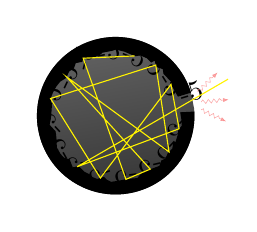
\begin{tikzpicture}[scale=1,rotate=10]
    \label{blackbody-cavity-reflection}

  \shade[top color=black!60,bottom color=black!80,shading angle=10] % background
    (7:1) arc (7:355:1);

  \fill[thick,black,postaction=decorate, % rough inner surface
    decoration={markings,mark=between positions 0.55 and 1 step 0.03 with {
                  \node[transform shape,inner sep=1pt]
                  (hit\pgfkeysvalueof{/pgf/decoration/mark info/sequence number}) {};
    }}]
    (7:1) arc (7:353:1) --++ (-7:-0.18)
    decorate[decoration={random steps,segment length=2,amplitude=1pt}]
        {arc (-7:-353:0.82)} -- cycle;

  \draw[yellow] % connect light ray to random points
    (8:1.5) -- (hit6.center) -- (hit1.center) -- (hit15.center) -- (hit5.center) --
    (hit9.center) -- (hit14.center) -- (hit2.center) -- (hit10.center) -- (hit3.center) --
    (hit4.center) -- (hit11.center) -- (hit13.center);

  \foreach \diagramAngle in {-35,-5,35}{
    \draw[cavity radiation] (1,0)++(\diagramAngle:0.1 and 0.2) --++ (\diagramAngle:0.35);
  }

\end{tikzpicture}

% BLACK BODY - without infalling light
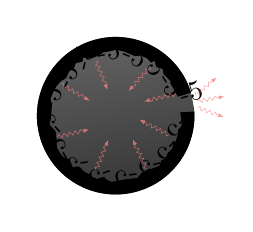
\begin{tikzpicture}[scale=1,rotate=10]
    \label{blackbody-cavity-emission}

  \shade[top color=black!60,bottom color=black!80,shading angle=10] % background
    (7:1) arc (7:355:1);

  \fill[thick,black,postaction=decorate, % rough inner surface
    decoration={markings,mark=between positions 0.55 and 1 step 0.03 with {
                  \node[transform shape,inner sep=1pt]
                  (hit\pgfkeysvalueof{/pgf/decoration/mark info/sequence number}) {};
    }}]
    (7:1) arc (7:353:1) --++ (-7:-0.18)
    decorate[decoration={random steps,segment length=2,amplitude=1pt}]
        {arc (-7:-353:0.82)} -- cycle;

  \foreach \diagramAngle [evaluate={\angin=\diagramAngle-180+10*rand; \r=0.76+0.05*rand; \l=0.4+0.02*rand}] in {10,45,100,140,190,240,290,330}{
    \draw[cavity radiation] (\diagramAngle:\r) --++ (\angin:\l);
  }

  \foreach \diagramAngle in {-30,0,30}{
    \draw[cavity radiation] (1,0)++(\diagramAngle:0.05 and 0.16) --++ (\diagramAngle:0.35);
  }

\end{tikzpicture}

% ref: https://tikz.net/blackbody_plots/
% Author: Izaak Neutelings (March 2019)
% BLACK BODY - 3000, 4000, 5000K
\begin{tikzpicture}
    \label{blackbody-spectra}
  \message{^^JBlack body}
  \def\N{60}
  \def\xmax{3100}
  \def\ymax{1.36e10}
  \def\tick#1#2{\draw[thick] (#1+.01*\ymax) -- (#1-.01*\ymax) node[below=-.5pt] {#2};}
  \begin{axis}[
      every axis plot/.style={
        mark=none,samples=\N,domain=5:\xmax,smooth},
      xmin=(-.05*\xmax), xmax=(1.05*\xmax),
      ymin=(-.08*\ymax), ymax=(1.08*\ymax),
      restrict y to domain=0:\ymax,
      axis lines=middle,
      axis line style=thick,
      %enlargelimits=upper, % extend the axes a bit to the right and top
      tick style={black,thick},
      %xtick style={draw=none},xticklabels=none,
      max space between ticks=26,
      xlabel={$\lambda/\unit{nm}$},
      ylabel={$B_\lambda/(\unit{\micro\watt\per\steradian\per\metre\squared\per\nano\metre})$},
      xlabel style={at={(rel axis cs:0.5,0)},below=-1pt},
      ylabel style={at={(rel axis cs:-0.11,0.5)},rotate=90},
      width=9cm, height=7cm,
      %clip=false
      tick scale binop=\times,
      every y tick scale label/.style={at={(rel axis cs:0,1)},anchor=south}
    ]

    % RAINBOW
    \shade[shading=rainbow,shading angle=90,opacity=0.5] (380,0) rectangle (740,\ymax);
    \node[above,inner sep=0pt] at (190,\ymax) {\strut UV}; % 10 - 400 nm
    \node[above,inner sep=0pt] at (560,\ymax) {\strut optical}; % 380 - 740 nm
    \node[above,inner sep=0pt] at (970,\ymax) {\strut IR}; % 740 - 1050 nm

    % PLANCK
    \addplot[very thick,red]    {planck(x,3000)};
    \addplot[very thick,orange] {planck(x,4000)};
    \addplot[very thick,samples=3*\N,blue] {planck(x,5000)};
    %\addplot[dashed,thick,red,domain=1000:4000]    {rayleighjeans(x,3000)};
    %\addplot[dashed,thick,orange,domain=1000:4000] {rayleighjeans(x,4000)};
    \addplot[dashed,thick,blue,domain=1000:4000]   {rayleighjeans(x,5000)};
    %\addplot[dashed,thick,red,domain=1000:4000]    {wien(x,3000)};
    %\addplot[dashed,thick,orange,domain=1000:4000] {wien(x,4000)};
    %\addplot[dashed,thick,blue,domain=1000:4000]   {wien(x,5000)};

    %% MAXIMUM (Wien's displacement law)
    %\addplot[mygreen,very thin,variable=T,domain=2500:6000]
    %  ({lampeak(T)},{planck(lampeak(T),T)});

    % LABELS
    \node[above=1pt,xshift=1.5pt,inner sep=0.5pt,red] at (1160,{planck(1160,3000)}) {\qty{3000}{K}};
    \node[above=4pt,xshift=2pt,inner sep=0.5pt,orange!80!black] at (930,{planck(930,4000)}) {\qty{4000}{K}};
    \node[above right=-1pt,blue] at (800,{planck(800,5000)}) {\qty{5000}{K}};
    \node[above right=-1pt,blue] at (1500,{rayleighjeans(1500,5000)}) {\qty{5000}{K} Rayleigh--Jeans};

    %% TICKS
    %\tick{500,0}{500}
    %\tick{1000,0}{1000}
    %\tick{1500,0}{1500}
    %\tick{2000,0}{2000}
    %\tick{2500,0}{2500}
    %\tick{3000,0}{3000}

  \end{axis}
\end{tikzpicture}


% BLACK BODY - 3000, 4000, 5000K, Wien's displacement law
\begin{tikzpicture}
    \label{blackbody-wien-displacement}
  \message{^^JBlack body, Wien's displacement law}
  \def\N{60}
  \def\xmax{3100}
  \def\ymax{1.36e10}
  \def\tick#1#2{\draw[thick] (#1+.01*\ymax) -- (#1-.01*\ymax) node[below=-.5pt] {#2};}
  \begin{axis}[
      every axis plot/.style={
        very thick,mark=none,samples=\N,domain=5:\xmax,smooth},
      xmin=(-.05*\xmax), xmax=(1.05*\xmax),
      ymin=(-.08*\ymax), ymax=(1.08*\ymax),
      restrict y to domain=0:\ymax,
      axis lines=middle,
      axis line style=thick,
      %enlargelimits=upper, % extend the axes a bit to the right and top
      tick style={black,thick},
      %xtick style={draw=none},xticklabels=none,
      max space between ticks=26,
      xlabel={$\lambda/\unit{nm}$},
      ylabel={$B_\lambda/(\unit{\micro\watt\per\steradian\per\metre\squared\per\nano\metre})$},
      xlabel style={at={(rel axis cs:0.5,0)},below=-1pt},
      ylabel style={at={(rel axis cs:-0.11,0.5)},rotate=90},
      width=9cm, height=7cm,
      %clip=false
      tick scale binop=\times,
      every y tick scale label/.style={at={(rel axis cs:0,1)},anchor=south}
    ]

    % RAINBOW
    \shade[shading=rainbow,shading angle=90,opacity=0.5] (380,0) rectangle (740,\ymax);
    \node[above,inner sep=0pt] at (190,\ymax) {\strut UV}; % 10 - 400 nm
    \node[above,inner sep=0pt] at (560,\ymax) {\strut optical}; % 380 - 740 nm
    \node[above,inner sep=0pt] at (970,\ymax) {\strut IR}; % 740 - 1050 nm

    % PLANCK
    \addplot[red]    {planck(x,3000)};
    \addplot[orange] {planck(x,4000)};
    \addplot[blue,samples=3*\N] {planck(x,5000)};
    \addplot[dashed,thick,blue,domain=1000:3500] {rayleighjeans(x,5000)};

    % MAXIMUM (Wien's displacement law)
    \addplot[mydarkgreen,thick,variable=T,domain=2200:4000,samples=40]
      ({lampeak(T)},{planck(lampeak(T),T)});
    \addplot[mydarkgreen,thick,variable=T,domain=4000:5200,samples=100]
      ({lampeak(T)},{planck(lampeak(T),T)});
    \fill[mydarkgreen!80!black] ({lampeak(3000)},{planck(lampeak(3000),3000)}) circle(1.5pt);
    \fill[mydarkgreen!80!black] ({lampeak(4000)},{planck(lampeak(4000),4000)}) circle(1.5pt);
    \fill[mydarkgreen!80!black] ({lampeak(5000)},{planck(lampeak(5000),5000)}) circle(1.5pt);

    % LABELS
    \node[above=1pt,xshift=1.5pt,inner sep=0.5pt,red] at (1160,{planck(1160,3000)}) {\qty{3000}{K}};
    \node[above=4pt,xshift=2pt,inner sep=0.5pt,orange!80!black] at (930,{planck(930,4000)}) {\qty{4000}{K}};
    \node[above right=-1pt,blue] at (800,{planck(800,5000)}) {\qty{5000}{K}};
    \node[above right=-1pt,blue] at (1500,{rayleighjeans(1500,5000)}) {\qty{5000}{K} Rayleigh--Jeans};

  \end{axis}
\end{tikzpicture}


% BLACK BODY - 3000, 4000, 5000K
\begin{tikzpicture}
    \label{blackbody-rayleigh-jeans}
  \message{^^JBlack body}
  \def\N{60}
  \def\xmax{3100}
  \def\ymax{1.43e10}
  \def\tick#1#2{\draw[thick] (#1+.01*\ymax) -- (#1-.01*\ymax) node[below=-.5pt] {#2};}
  \begin{axis}[
      every axis plot/.style={
        mark=none,samples=\N,domain=5:\xmax,smooth},
      xmin=(0), xmax=(\xmax),
      ymin=(0), ymax=(\ymax),
      restrict y to domain=0:\ymax,
      %axis lines=middle,
      axis line style=thick,
      tick style={black,thick},
      xlabel={$\lambda/\unit{nm}$},
      ylabel={$B_\lambda/(\unit{\micro\watt\per\steradian\per\metre\squared\per\nano\metre})$},
      xlabel style={below=-1pt},
      ylabel style={above=-1pt},
      width=9cm, height=7cm,
      tick scale binop=\times,
      every y tick scale label/.style={at={(rel axis cs:0,1)},anchor=south}
    ]

    % RAINBOW
    \draw[dashed] (380,{planck(380,5000)}) -- (380,.90*\ymax);
    \draw[dashed] (740,{planck(740,5000)}) -- (740,.90*\ymax);
    \begin{scope}
      \clip[variable=\x,domain=200:1000,samples=40]
        plot(\x,{planck(\x,5000)}) |- (200,0) -- cycle;
      \shade[shading=rainbow,shading angle=90,opacity=0.7] (380,0) rectangle (740,\ymax);
    \end{scope}

    % PLANCK
    \addplot[very thick,red]    {planck(x,3000)};
    \addplot[very thick,orange] {planck(x,4000)};
    \addplot[very thick,samples=3*\N,blue] {planck(x,5000)};
    \addplot[dashed,thick,blue,domain=1000:4000]   {rayleighjeans(x,5000)};

    % MAXIMUM (Wien's displacement law)
    \addplot[mydarkgreen,thick,variable=T,domain=2200:4000,samples=40]
      ({lampeak(T)},{planck(lampeak(T),T)});
    \addplot[mydarkgreen,thick,variable=T,domain=4000:5000,samples=100]
      ({lampeak(T)},{planck(lampeak(T),T)});
    \fill[mydarkgreen!80!black] ({lampeak(3000)},{planck(lampeak(3000),3000)}) circle(1.5pt);
    \fill[mydarkgreen!80!black] ({lampeak(4000)},{planck(lampeak(4000),4000)}) circle(1.5pt);
    \fill[mydarkgreen!80!black] ({lampeak(5000)},{planck(lampeak(5000),5000)}) circle(1.5pt);

    % LABELS
    \node[above=1pt,xshift=1.5pt,inner sep=0.5pt,red]
      at (1160,{planck(1160,3000)}) {\qty{3000}{K}};
    \node[above=4pt,xshift=2pt,inner sep=0.5pt,orange!80!black]
      at (930,{planck(930,4000)}) {\qty{4000}{K}};
    \node[above right=-1pt,blue]
      at (800,{planck(800,5000)}) {\qty{5000}{K}};
    \node[above right=-1pt,blue]
      at (1500,{rayleighjeans(1500,5000)}) {\qty{5000}{K} Rayleigh--Jeans};

    % LABELS
    \node[below=2pt] at (200,\ymax) {\strut UV}; % 10 - 400 nm
    \node[below=2pt] at (562,\ymax) {\strut optical}; % 380 - 740 nm
    \node[below=2pt] at (920,\ymax) {\strut IR}; % 740 - 1050 nm

  \end{axis}
\end{tikzpicture}


% BLACK BODY LOG-LOG - colors
% See https://tikz.net/blackbody_color/
\begin{tikzpicture}
    \label{blackbody-spectra-log} %[scale=2]
  \message{^^JBlack body colors}
  \def\N{40}
  \def\xmin{35}
  \def\xmax{1.7e5}
  \def\ymin{1e2}
  \def\ymax{2e12}
  \begin{loglogaxis}[
      every axis plot post/.append style={
        very thick,mark=none,domain=\xmin:\xmax,samples=\N,smooth},
      xmin=\xmin, xmax=(1.01*\xmax),
      ymin=\ymin, ymax=\ymax,
      restrict y to domain=0.1*\ymin:\ymax,
      log basis y=10,
      axis line style=thick,
      tick style={black,thick},
      max space between ticks=23,
      yminorticks=false,
      xlabel={$\lambda/\unit{nm}$},
      ylabel={$B_\lambda/(\unit{\micro\watt\per\steradian\per\metre\squared\per\nano\metre})$},
      ylabel style={above=-2pt},
      legend style={at={(1.02,0.5)},anchor=west,draw=none,fill=none},
      legend cell align={left},
      width=8cm, height=6cm,
      axis line on top
    ]

    % RAINBOW
    \shade[shading=rainbow,shading angle=90,opacity=0.5] (380,\ymin) rectangle (740,\ymax);

    % PLANCK
    \addplot[10000K] {planck(x,10000)};
    \addplot[6000K]  {planck(x,7500)};
    \addplot[5000K]  {planck(x,5000)};
    \addplot[3000K]  {planck(x,3000)};
    \addplot[2000K]  {planck(x,2000)};
    \addplot[1000K]  {planck(x,1000)};
    \addplot[black]  {planck(x, 500)};
    %\addplot[dashed,thick,black] {rayleighjeans(x,500)};

    % LEGENDS
    \addlegendentry{\qty{10000}{K}}
    \addlegendentry{\qty{7500}{K}}
    \addlegendentry{\qty{5000}{K}}
    \addlegendentry{\qty{3000}{K}}
    \addlegendentry{\qty{2000}{K}}
    \addlegendentry{\qty{1000}{K}}
    \addlegendentry{\qty{500}{K}}

  \end{loglogaxis}
\end{tikzpicture}


% BLACK BODY LOG-LOG - Rayleigh-Jeans / Wien, 300K
\begin{tikzpicture}
    \label{blackbody-approximations-300k}
  \message{^^JRayleigh-Jeans / Wien, 300K}
  \def\N{40}
  \def\xmin{1.5e3}
  \def\xmax{2e6}
  \def\ymin{5e-4}
  \def\ymax{3e4}
  \begin{loglogaxis}[
      every axis plot/.style={
        very thick,mark=none,domain=\xmin:\xmax,samples=\N,smooth},
      xmin=\xmin, xmax=(1.01*\xmax),
      ymin=\ymin, ymax=\ymax,
      restrict y to domain=0.1*\ymin:\ymax,
      log basis y=10,
      axis line style=thick,
      tick style={black,thick},
      %ticks=none,
      max space between ticks=23,
      yminorticks=false,
      xlabel={$\lambda/\unit{nm}$},
      ylabel={$B_\lambda/(\unit{\micro\watt\per\steradian\per\metre\squared\per\nano\metre})$},
      ylabel style={above=-2pt},
      width=8cm, height=6cm,
      legend style={at={(0.14,0.15)},anchor=south west,draw=none,fill=none},
      legend cell align={left},
      axis line on top
    ]

    % PLANCK
    \addplot[black]      {planck(x,300)};
    \addplot[thick,blue] {rayleighjeans(x,300)};
    \addplot[thick,red]  {wien(x,300)};

    % LEGENDS
    \addlegendentry{Planck}
    \addlegendentry{Rayleigh--Jeans}
    \addlegendentry{Wien}
    \node at (0.18*\xmax,0.01*\ymax) {$T = \qty{300}{K}$};

  \end{loglogaxis}
\end{tikzpicture}


% BLACK BODY LOG-LOG - Rayleigh-Jeans / Wien, 3000K
\begin{tikzpicture}
    \label{blackbody-approximations-3000k}
  \message{^^JRayleigh-Jeans / Wien, 3000K}
  \def\N{40}
  \def\xmin{1.5e2}
  \def\xmax{2e5}
  \def\ymin{5e1}
  \def\ymax{4e9}
  \begin{loglogaxis}[
      every axis plot/.style={
        very thick,mark=none,domain=\xmin:\xmax,samples=\N,smooth},
      xmin=\xmin, xmax=(1.01*\xmax),
      ymin=\ymin, ymax=\ymax,
      restrict y to domain=0.1*\ymin:\ymax,
      log basis y=10,
      axis line style=thick,
      tick style={black,thick},
      %ticks=none,
      max space between ticks=23,
      yminorticks=false,
      xlabel={$\lambda/\unit{nm}$},
      ylabel={$B_\lambda/(\unit{\micro\watt\per\steradian\per\metre\squared\per\nano\metre})$},
      ylabel style={above=-2pt},
      width=8cm, height=6cm,
      legend style={at={(0.14,0.15)},anchor=south west,draw=none,fill=none},
      legend cell align={left},
      axis line on top
    ]

    % RAINBOW
    \shade[shading=rainbow,shading angle=90,opacity=0.1] (380,\ymin) rectangle (740,\ymax);

    % PLANCK
    \addplot[black]      {planck(x,3000)};
    \addplot[thick,blue] {rayleighjeans(x,3000)};
    \addplot[thick,red]  {wien(x,3000)};

    % LEGENDS
    \addlegendentry{Planck}
    \addlegendentry{Rayleigh--Jeans}
    \addlegendentry{Wien}
    \node at (0.17*\xmax,0.01*\ymax) {$T = \qty{3000}{K}$};

  \end{loglogaxis}
\end{tikzpicture}


% BLACK BODY LOG-LOG - Rayleigh-Jeans / Wien
\begin{tikzpicture}
    \label{blackbody-approximations}
  \message{^^JRayleigh-Jeans / Wien}
  \def\N{40}
  \def\xmin{3e2}
  \def\xmax{2e6}
  \def\ymin{1e-3}
  \def\ymax{1e7}
  \begin{loglogaxis}[
      every axis plot/.style={
        very thick,mark=none,domain=\xmin:\xmax,samples=\N,smooth},
      xmin=\xmin, xmax=(1.01*\xmax),
      ymin=\ymin, ymax=\ymax,
      restrict y to domain=0.1*\ymin:\ymax,
      log basis y=10,
      axis line style=thick,
      tick style={black,thick},
      %ticks=none,
      max space between ticks=23,
      yminorticks=false,
      xlabel={$\lambda/\unit{nm}$},
      ylabel={$B_\lambda/(\unit{\micro\watt\per\steradian\per\metre\squared\per\nano\metre})$},
      ylabel style={above=-2pt},
      width=8cm, height=6cm,
      axis line on top,
      legend style={at={(0.65,0.9)},anchor=north west,draw=none,fill=none}%,
      %legend cell align={left},
    ]

    % RAINBOW
    \shade[shading=rainbow,shading angle=90,opacity=0.5] (380,\ymin) rectangle (740,\ymax);

    % PLANCK
    \addplot[blue]  {planck(x,800)};
    \addplot[red]   {planck(x,300)};
    \addplot[black] {planck(x,100)};
    \addplot[dashed,thick,black] {rayleighjeans(x,100)};
    \addplot[dashed,thick,red]   {rayleighjeans(x,300)};
    \addplot[dashed,thick,blue]  {rayleighjeans(x,800)};
    \addplot[dotted,thick,black] {wien(x,100)};
    \addplot[dotted,thick,red]   {wien(x,300)};
    \addplot[dotted,thick,blue]  {wien(x,800)};

    % LEGENDS
    \addlegendentry{\qty{800}{K}}
    \addlegendentry{\qty{300}{K}}
    \addlegendentry{\qty{100}{K}}

  \end{loglogaxis}
\end{tikzpicture}


% BLACK BODY LOG-LOG - CMB redshift
\begin{tikzpicture}
    \label{blackbody-cmb-redshift}
  \message{^^JCMB redshift}
  \def\N{60}
  \def\xmin{5e1}
  \def\xmax{2e8}
  \def\ymin{1e-10}
  \def\ymax{1e11}
  \begin{loglogaxis}[
      every axis plot/.style={
        very thick,mark=none,samples=\N,smooth},
      xmin=\xmin, xmax=(1.01*\xmax),
      ymin=\ymin, ymax=\ymax,
      restrict y to domain=0.1*\ymin:\ymax,
      log basis y=10,
      axis line style=thick,
      tick style={black,thick},
      %ticks=none,
      max space between ticks=23,
      yminorticks=false,
      variable=x,
      xlabel={$\lambda/\unit{nm}$},
      ylabel={$B_\lambda/(\unit{\micro\watt\per\steradian\per\metre\squared\per\nano\metre})$},
      ylabel style={above=-2pt},
      width=8cm, height=6cm,
      axis line on top
    ]

    % BANDS
    % See https://tikz.net/electromagnetic_spectrum/
    \fill[violet!80!black!5] (\xmin,\ymin) rectangle (380,\ymax); % ultraviolet
    \shade[shading=rainbow,shading angle=90,opacity=0.5] (380,\ymin) rectangle (740,\ymax);
    \fill[red!80!black!4] (740,\ymin) rectangle (1e6,\ymax); % infrared
    \fill[orange!80!black!4] (1e6,\ymin) rectangle (1e8,\ymax); % microwave
    \fill[green!80!black!4] (1e8,\ymin) rectangle (\xmax,\ymax); % radio
    \node[below=3,violet!50!black] at ({\xmin*10^(log10(380/\xmin)/2)},\ymax) {UV};
    \node[below=3,red!50!black] at ({740*10^(log10(1e6/740)/2)},\ymax) {infrared};
    \node[below=3,orange!60!black] at ({1e6*10},\ymax) {microwave};

    % PLANCK
    \addplot[domain=\xmin:1e5,red]     {planck(x,3000)};
    \addplot[domain=1e5:\xmax,red]     {rayleighjeans(x,3000)}; % prevent rounding errors in tail
    \addplot[domain=2e5:\xmax,mygreen] {planck(x,2.725)};

    % LABELS
    \node[above right=1pt,red] at (4e4,{planck(4e4,3000)}) {\qty{3000}{K}};
    \node[anchor=-70,mygreen] at (1e6,{planck(1e6,2.725)}) {\qty{2.725}{K}};

    % ARROW
    \draw[->,line width=2,myred] (7e3,1e2) --++ (-42:17mm)
      node[pos=0.38,above,sloped] {redshift}
      node[pos=0.38,below,sloped] {$z \sim 1100$};

  \end{loglogaxis}
\end{tikzpicture}


% BLACK BODY LOG-LOG - CMB temperature variations
% https://en.wikipedia.org/wiki/Cosmic_microwave_background#Relationship_to_the_Big_Bang
% T ~ 2.725 K with anisotropic variations of ~ 18 uK = 0.000018 K
\begin{tikzpicture}
    \label{blackbody-cmb-variation}
  \message{^^JCMB temperature variations}
  \def\N{40}
  \def\xmin{3.2e5}
  \def\xmax{8e6}
  \def\ymin{5e-9}
  \def\ymax{1e-6}
  \begin{loglogaxis}[
      every axis plot post/.append style={
        very thick,mark=none,samples=\N,domain=\xmin:\xmax,smooth},
      xmin=\xmin, xmax=(1.01*\xmax),
      ymin=\ymin, ymax=\ymax,
      restrict y to domain=0.1*\ymin:\ymax,
      log basis y=10,
      axis line style=thick,
      tick style={black,thick},
      xtick={5e5,1e6,2e6,5e6},
      minor xtick={4e5,6e5,7e5,8e5,9e5,3e6,4e6,6e6},
      log number format code/.code={
        \pgfkeys{/pgf/fpu}
        \pgfmathparse{exp(\tick)}
        \pgfmathprintnumber[sci,sci zerofill,precision=0]{\pgfmathresult}
        \pgfkeys{/pgf/fpu=false}
      },
      xlabel={$\lambda/\unit{nm}$},
      ylabel={$B_\lambda/(\unit{\micro\watt\per\steradian\per\metre\squared\per\nano\metre})$},
      ylabel style={above=-2pt},
      width=8cm, height=6cm,
      axis line on top,
      legend style={
        at={(0.24,0.3)},anchor=south west,draw=none,fill=none},
      legend cell align={left},
      legend image code/.code={
        \draw[mark repeat=2,mark phase=2]
        plot coordinates {(0cm,0cm) (0.28cm,0cm) (0.56cm,0cm)};%
      }
    ]

    % PLANCK
    \addplot[red,dashed]  {planck(x,2.750)};
    \addplot[mygreen]     {planck(x,2.725)};
    \addplot[blue,dashed] {planck(x,2.700)};
    \addplot[red,dashed]  {planck(x,2.750)}; % draw over 2.725

    % LEGENDS
    \addlegendentry{\qty{2.750}{K}}
    \addlegendentry{\qty{2.725}{K}}
    \addlegendentry{\qty{2.700}{K}}

  \end{loglogaxis}
\end{tikzpicture}

% ref: https://tikz.net/blackbody_color/
% author: Izaak Neutelings (March 2019)
% RAINBOW

\begin{tikzpicture}
    \label{visible-spectrum}
  \shade[shading=rainbow,shading angle=270] (0,0) rectangle (10,1);
\end{tikzpicture}


% BLACK BODY
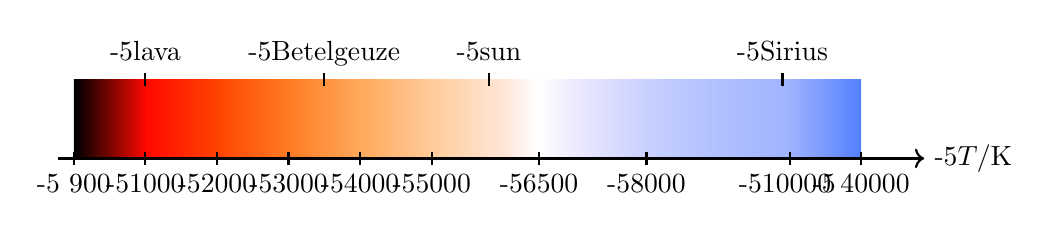
\begin{tikzpicture}
    \label{blackbody-colors}

  \def\tick#1#2{\draw[thick] (#1+.08) --++ (0,-.16) node[below=-2pt] {\strut #2};}
  \def\ticka#1#2{\draw[thick] (#1+.08) --++ (0,-.16) node[above=2pt] {\strut #2};}

  %   i  TEMPERATURE  RGB COLOR
  %   0        900    0.0000 0.0000 0.0000
  %  10       1000    1.0000 0.0337 0.0000
  %  20       2000    1.0000 0.2647 0.0033
  %  30       3000    1.0000 0.4870 0.1411
  %  40       4000    1.0000 0.6636 0.3583
  %  50       5000    1.0000 0.7992 0.6045
  %  60       6000    1.0000 0.9019 0.8473
  %           6500    0.9997 0.9998 1.0000 white
  %  70       7000    0.9337 0.9150 1.0000
  %  80       8000    0.7874 0.8187 1.0000
  %  90       9000    0.6925 0.7522 1.0000
  %          10000    0.6268 0.7039 1.0000
  %          15000    0.4749 0.5824 1.0000
  %          30000    0.3751 0.4926 1.0000
  % 100      40000    0.3277 0.5022 1.0000
  % http://www.vendian.org/mncharity/dir3/blackbody/UnstableURLs/bbr_color.html

  \shade[shading=blackbody,shading angle=-90] (0,0) rectangle (10,1);
  \draw[->,thick] (-0.2,0) -- (10.8,0) node[right] {$T/\unit{K}$};
  \tick{0,0}{ 900}
  \tick{10/11*1,0}{1000}
  \tick{10/11*2,0}{2000}
  \tick{10/11*3,0}{3000}
  \tick{10/11*4,0}{4000}
  \tick{10/11*5,0}{5000}
  \tick{10/11*6.5,0}{6500}
  \tick{10/11*8,0}{8000}
  \tick{10/11*10,0}{10000\,\,}
  \tick{10,0}{\,40000}

  % EXAMPLES
  \ticka{10/11*1.0,1}{\strut lava}
  \ticka{10/11*3.5,1}{\strut Betelgeuze}
  \ticka{10/11*5.8,1}{\strut sun}
  \ticka{10/11*9.9,1}{\strut Sirius}

\end{tikzpicture}

\begin{tikzpicture}[>=Latex,
    light/.style={thick,blue!65!black,->},
    readout/.style={draw=ink,rounded corners=1.5pt,fill=ink!4,inner sep=3pt}]
    \label{hom-ports}
    \coordinate (bs) at (0,0);
    \node[left] (a) at (-3.5,0) {$a$};
    \node[below] (b) at (0,-1.35) {$b$};
    \node[draw=ink,fill=white] (delay) at (0,-.72) {延迟 $\tau$};
    \node[readout] (c) at (3.1,0) {探测器 $c$};
    \node[readout] (d) at (0,1.45) {探测器 $d$};
    \node[readout] (both) at (3.1,1.45) {符合计数};
    \draw[light] (a.east) -- (bs);
    \draw[light] (b.north) -- (delay.south);
    \draw[light] (delay.north) -- (bs);
    \draw[light] (bs) -- (c.west);
    \draw[light] (bs) -- (d.south);
    \draw[teal!70!black,line width=1.6pt,dashed] (-.32,-.32) -- (.32,.32);
    \node[above left] at (-.12,.1) {平衡分束器};
    \draw[->] (c.north) -- (both.south);
    \draw[->] (d.east) -- (both.west);
\end{tikzpicture}

\end{document}
